\documentclass{article}

% if you need to pass options to natbib, use, e.g.:
\PassOptionsToPackage{numbers, compress}{natbib}
% before loading neurips_2026

% The authors should use one of these tracks.
% Before accepting by the NeurIPS conference, select one of the options below.
% 0. "default" for submission
\usepackage{tabularx}
\usepackage{xcolor}
% the "default" option is equal to the "main" option, which is used for the Main Track with double-blind reviewing.
\usepackage{fvextra} % for Unicode in verbatim
% 1. "main" option is used for the Main Track
%  \usepackage[main]{neurips_2026}
% 2. "position" option is used for the Position Paper Track
%  \usepackage[position]{neurips_2026}
% 3. "eandd" option is used for the Evaluations & Datasets Track
 % \usepackage[eandd]{neurips_2026}
% 4. "creativeai" option is used for the Creative AI Track
%  \usepackage[creativeai]{neurips_2026}
% 5. "sglblindworkshop" option is used for the Workshop with single-blind reviewing
 % \usepackage[sglblindworkshop]{neurips_2026}
% 6. "dblblindworkshop" option is used for the Workshop with double-blind reviewing
  \usepackage[dblblindworkshop]{neurips_2026}
% 7. "education" option is used for the Education Track
%  \usepackage[education]{neurips_2026}

\usepackage{todonotes}
\setuptodonotes{size=\tiny}

% After being accepted, the authors should add "final" behind the track to compile a camera-ready version.
% 1. Main Track
 % \usepackage[main, final]{neurips_2026}
% 2. Position Paper Track
%  \usepackage[position, final]{neurips_2026}
% 3. Evaluations & Datasets Track
 % \usepackage[eandd, final]{neurips_2026}
% 4. Creative AI Track
%  \usepackage[creativeai, final]{neurips_2026}
% 5. Workshop with single-blind reviewing
%  \usepackage[sglblindworkshop, final]{neurips_2026}
% 6. Workshop with double-blind reviewing
%  \usepackage[dblblindworkshop, final]{neurips_2026}
% Note. For the workshop paper template, both \title{} and \workshoptitle{} are required, with the former indicating the paper title shown in the title and the latter indicating the workshop title displayed in the footnote.
% For workshops (5., 6.), the authors should add the name of the workshop, "\workshoptitle" command is used to set the workshop title.
\workshoptitle{NeurIPS 2026 Workshop on World Models in Physical AI}
% 7. Education Track
% \usepackage[education, final]{neurips_2026}

% "preprint" option is used for arXiv or other preprint submissions
 % \usepackage[preprint]{neurips_2026}

% to avoid loading the natbib package, add option nonatbib:
%    \usepackage[nonatbib]{neurips_2026}

\usepackage[utf8]{inputenc} % allow utf-8 input
\usepackage[T1]{fontenc}    % use 8-bit T1 fonts
\usepackage{hyperref}       % hyperlinks
\usepackage{url}            % simple URL typesetting
\usepackage{booktabs}       % professional-quality tables
\usepackage{amsfonts}       % blackboard math symbols
\usepackage{nicefrac}       % compact symbols for 1/2, etc.
\usepackage{microtype}      % microtypography
\usepackage{xcolor}         % colors

\usepackage{amsmath}

\usepackage{todonotes}
\setuptodonotes{size=\tiny}


% Note. For the workshop paper template, both \title{} and \workshoptitle{} are required, with the former indicating the paper title shown in the title and the latter indicating the workshop title displayed in the footnote. 
\title{Mechanical Validity Does Not Imply Structural Fidelity in LLM-Generated Executable POSGs}


% The \author macro works with any number of authors. There are two commands
% used to separate the names and addresses of multiple authors: \And and \AND.
%
% Using \And between authors leaves it to LaTeX to determine where to break the
% lines. Using \AND forces a line break at that point. So, if LaTeX puts 3 of 4
% authors names on the first line, and the last on the second line, try using
% \AND instead of \And before the third author name.


\author{Anonymous Authors}


\begin{document}


\maketitle


\begin{abstract}
  %The abstract paragraph should be indented \nicefrac{1}{2}~inch (3~picas) on both the left- and right-hand margins. Use 10~point type, with a vertical spacing (leading) of 11~points. The word \textbf{Abstract} must be centered, bold, and in point size 12. Two line spaces precede the abstract. The abstract must be limited to one paragraph.
Executable world models used for planning must preserve action-conditioned dynamics, not merely satisfy a software interface. We evaluate LLM-generated partially observable stochastic games (POSGs) with a 44-scenario benchmark that separates mechanical validity, permutation-invariant structural matching, and semantic diagnostics. Across three empirical tracks we analyze 354 completed first-pass candidates. In the reference-backed game track, 134/135 final artifacts pass a strict post-hoc mechanical audit, yet their mean permutation-invariant structural F1 is 0.3660 (median 0.1778), and only 28/134 score exactly 1. Across the three observed generations per LLM--game pair, the mean within-pair F1 standard deviation is 0.1679, while an exploratory nine-game analysis associates reference stochasticity with lower agreement ($\rho=-0.677$). These results show that executability is a necessary gate but does not establish structural fidelity.
\end{abstract}

\section{Introduction}
\label{sec:intro}
\paragraph{Motivation and Core Challenge}
% \todo{i'm not sure "formatting" is the right phrase. also, i'm not sure "safe-by-design" is essential. what if we use the title "Can LLMs Construct Formal, Situational World Models for AI Agents? Test Cases, Evaluation Methods, and First Results"}
% \todo{make sure all official general neurips and workshop-specific formatting rules are followed!}
% \todo{we must agree on an author list and ordering since that is probably part of the online submission form. i suggest alphabetical ordering for simplicity, unless someone vetos this.}
Many approaches to ``safe-by-design'' AI systems \citep{dalrymple2024guaranteedsafeaiframework} rely on formal, tractable world models to evaluate safety-critical metrics such as action reversibility \citep{eysenbach2018leave}, state reachability \citep{krakovna2020avoiding}, agent empowerment \citep{klyubin2005empowerment}, or the effects on capabilities and resulting (dis)empowerment of the humans an agent interacts with \citep{salge2017empowerment,heitzigfair}. 
Traditional world models such as neural network approximations or large Bayesian networks \citep{amodei2016concrete,ha2018world} often lack structural transparency and/or symbolic grounding required for formal verification  \citep{konidaris2018from}, or are too large for tractable planning. 

Generating formal, ``situational world models'' that are suitable for a given situation and a given level of granularity of the decision making process just in time is a possible way to address transparency and tractability.
A significant challenge for such an approach is that the suitability criteria for a situational world model depend on the specific context. In industrial, single-agent planning scenarios with predominantly deterministic dynamics, suitability mostly means correctness and is relatively easy to assess: the world model either accurately represents the environment's mechanics at the given level of detail, or it does not, and its predictions can often be verified against the actual dynamics.

In complex real-world situations with several individuals, such clarity often fades. There is not just one accurate world model---various plausible world models emphasize different stakeholders, choices, and outcomes. It becomes easy to overlook an ethically significant aspect: a party involved may not take explicit action, an option might only be significant under uncertain cultural norms, and a consequence, while unlikely, may be severe. In this situation, assessing the balance between tractability and sufficient detail is challenging. If the world model is too simple, it might miss the key distinction on which the safe action depends, and there is no ground-truth reference available against which to detect the loss.

Addressing this trade-off might require a hierarchical approach, where situations are described at multiple levels of granularity and refined only on demand. %where safety-relevant distinctions demand it. 
In this paper, we focus on a single layer of such a hierarchy: generating and evaluating one situational world model per scenario.
% \todo{i like this very much so far!}

\paragraph{LLMs as World Model Generators}
This work investigates whether modern Large Language Models (LLMs) can bridge the gap between unstructured, real-world scenario descriptions and formal safety environments by constructing Partially Observable Stochastic Games (POSGs) encoded in a structured format (JSON or Python). For single-agent, largely deterministic settings, literature shows that LLMs are able to produce correct world models expressed in planning languages such as PDDL, and to generate executable ``code world models'' for model-based planning \citet{cao2025large,dainese2024generating}. For complex situations with multiple affected humans, this capability has been studied far less, and arguably PDDL or its extensions might not (yet) be the right data structures to represent them.
%
The multi-human setting also faces failure modes that are specific to LLM generation and largely absent from the deterministic single-agent case:
\begin{itemize}
    \item \textbf{Invention of details:} the world model introduces facts, quantities, or intentions that are absent from the situation description, such as an invented feature, a freely made-up probability, an attributed goal, or a fabricated participant. If the formal schema (e.g. a fully instead of partially observed stochastic game, or the requirement to specify ``rewards'') requires commitment to quantities the text underdetermines, this failure is invited rather than incidental.
    \item \textbf{Omission of inferable structure:} the world model overlooks a stakeholder, state variable, or behavioral option that is not explicitly mentioned but that general world understanding would recognize as plausibly present and safety-relevant. For example, a custodial party who never acts explicitly but whose interests determine the safe outcome.
    \item \textbf{Bias, especially under cultural uncertainty:} when the situation leaves the cultural context underspecified, the world model may resolve it according to a dominant prior, systematically privileging particular interpretations. On the other hand, when a cultural context is specified, the world model might take up clich\'ees and preconceptions from the LLM's training data.
\end{itemize}

These are not merely syntactic or mechanical quality failures. Each can occur in an otherwise well-formed world model while materially changing the conclusions of a downstream planner. This distinction motivates our evaluation framework: mechanical validity alone is insufficient, and evaluation must additionally test structural fidelity, semantic coverage, and unsupported invention.

\paragraph{Key Contributions}
In this workshop paper, we contribute:
\begin{itemize}
    \item A curated corpus of 44 test-case situations spanning toy, game, situational, and cultural scenarios, tiered by how much ground truth is available.
    \item A generation pipeline that prompts LLMs to produce POSG world models in a structured JSON schema or as python classes implementing a given abstract base class.
    \item A multi-lane evaluation framework separating mechanical validity, reference-backed structural comparison, and diagnostic semantic coverage.
    \item Three empirical tracks: reference-backed games, open-ended situational Python POSGs, and culturally contextualized JSON POSGs, with explicit evidence boundaries for each.
\end{itemize}


\section{Related Work}
\label{sec:related_work}

\paragraph{Safe-by-Design AI and Empowerment}
%Formal safety criteria require explicit modeling of state-action-state transitions to ensure non-irreversible actions and maintain bounded agent influence.
A line of work aims to keep AI systems safe by preserving human choices rather than telling AI agents what to do. Methods like attainable-utility preservation \citep{turner2020conservative} and reachability-based side-effect penalties \citep{krakovna2020avoiding} aim to make AI agents act cautiously, but quantify this from the agent's own perspective rather than measuring human capability. In contrast, empowerment-based goals aim to preserve or increase the human's capability to influence outcomes. Recent research formalises a fair, risk- and inequality-averse aggregate of human power as a formal AI objective \citet{heitzigfair}. All these methods rely on a clear state–action–state framework: computing reversibility, reachability, or power presupposes a world model that already contains the relevant stakeholders, options, and consequences. This makes the quality of a generated world model a safety concern rather than a modelling convenience, and what our evaluation is designed to check.

\paragraph{LLMs for Environment Synthesis and Code Generation}
%Prior research explores generating grid-worlds or domain-specific languages (DSLs) via LLMs, but lacks comprehensive multi-agent stochastic game modeling.
LLMs have been used to synthesize environments and domain-specific programs, including generating grid worlds, task specifications, and planning-language descriptions. \citet{dainese2024generating} generated code-world models (Python implementations of an environment's dynamics) for model-based reinforcement learning. They argue that calling code at planning time, rather than an LLM, yields greater precision, interpretability, and efficiency, and they validate the generated code against unit tests and environment trajectories. \citet{cao2025large} survey the broader LLM planning literature, categorizing methods into external-module-augmented, finetuning-based, and search-based approaches. This work focuses on single-agent settings and assumes access to a ground truth (an executable environment or a verifiable plan) against which generated artifacts can be evaluated. Our problem setting differs on both assumptions: we consider a multi-player (AIs and humans) stochastic game, and in realistic applications there is no ground-truth world model to validate against, which motivates the evaluation design in Section~\ref{subsec:evaluation_framework}.

\paragraph{World Model Evaluation}
%Discussion of existing benchmarking tools for state-space coverage, LLM-as-a-judge reliability, and structural graph analysis in synthetic environments.
Evaluating synthesised situational world models draws on several metrics, including mechanical validity checks (well-formedness, probability normalisation, reachability), structural and graph-based comparison of state-transition topologies, and LLM-as-a-judge protocols for qualities that are difficult to verify automatically. Existing metrics often assume the existence of a reference world model, failing to address situations where correctness is genuinely indeterminate and must be evaluated against human-specified expectations rather than a ground-truth world model. We combine mechanical, structural, and judgement-based metrics into a single framework in Section~\ref{subsec:evaluation_framework}.

\section{Benchmark and World Model Generation}
\label{sec:method}

%\subsection{POSG representation}
\label{subsec:preliminaries}

\paragraph{Partially Observable Stochastic Games (POSG)}
A formal POSG is defined as a tuple $\mathcal{M} = \langle \mathcal{N}, \mathcal{S}, \mathcal{A}=\{\mathcal{A}_i\}_{i \in \mathcal{N}}, \mathcal{P}, \mathcal{O}=\{\mathcal{O}_i\}_{i \in \mathcal{N}}, \Omega \rangle$, where $\mathcal{N}$ is a set of players which may include humans and AI systems,
%\todo{let's use the established game-theoretical term `player' for humans+AIs, and reserve `agent' for AI systems?}
$\mathcal{S}$ is the set of (potentially hidden) states, $\mathcal{A}_i$ is the action space for player $i$, $\mathcal{P}(s' \mid s, a)$ defines state transition probabilities given joint action $a=\{a_i\}_{i\in\mathcal N}$, and $\Omega:\mathcal S\times\mathcal A\times\mathcal S\to\mathcal O$ is a (deterministic) observation function representing what every player will actually observe after a transition.

\paragraph{The Situation--World Model--Planner Architecture}
We adopt a modular, neutral baseline architecture decoupling the world model from policy synthesis:
\begin{enumerate}
    \item \textbf{Perception / Prompt Input}: The natural-language scenario or situation description.
    \item \textbf{Situational World Model (LLM Output)}: A neutral, predictive resource representing valid state-space transitions without embedded agent biases.
    \item \textbf{Planner / Decision Engine}: The downstream decision algorithm executing policy searches over the synthesized world model (e.g. some form of dynamic programming or model-based reinforcement learning).
\end{enumerate}

\paragraph{Output Formats for Representing Situational World Models}
World models are formalized as POSGs encoded either as explicit JSON structures listing individual transitions, obeying a prescribed schema (for small state spaces), or as executable Python classes generating transitions programmatically, extending a prescribed Abstract Base Class (for more complex environments).
% \todo{I also like sections 2 and 3 very much so far! you're on a good track!!}

% \begin{figure}
%     \centering
%     \includegraphics[width=1\linewidth]{world model generation.png}
%     \caption{World-Model Generation.}
%     \label{fig:world}
% \end{figure}

%\subsection
\paragraph{Benchmark suite}
\label{sec:dataset}

To evaluate world model synthesis, we construct a specialized benchmark suite that prioritizes structural diversity, domain coverage, and distinct multi-player trade-offs over brute-force data volume. Rather than inflating dataset size through trivial parameter variations—such as resizing grids or swapping entity labels—each scenario introduces a unique combination of partial observability, state-space topology, non-zero-sum payoff structure, and safety-critical choices.

The dataset has four domain tiers, designed to isolate specific reasoning challenges ranging from transition dynamics to normative constraints:
(1) 10 {\bf toy environments} with tightly specified mechanics; (2) 9 simple {\bf games} with known rules and reference structure; (3) 11 {\bf situational} scenarios involving asymmetric stakeholders, resources, or consequences; and (4) 14 {\bf culturally contextualized} scenarios in which relevant structure or norms may be underspecified.
%%%%%%%%%%%%%%%%%% deactivated for space and since the state space and action space counts are misleading into thinking there was a ground truth!
\iffalse
To provide a granular view of the dataset's scope, Table~\ref{tab:dataset_taxonomy} outlines the scenario distribution across all four categories, detailing the explicit case counts and representative state-action dimensions.
\begin{table*}[t]
\centering
\small
\caption{Taxonomy of the benchmark suite detailing scenario counts, state-space scale ($|S|$), and action-space dimensionality ($|A|$) across tiers.}
\label{tab:dataset_taxonomy}
\begin{tabularx}{\linewidth}{l X c c c}
\toprule
\textbf{Tier} & \textbf{Category} & \textbf{Count} & \textbf{State Space $|S|$} & \textbf{Action Space $|A|$} \\
\midrule
\textbf{01} & Toy Environments & 10 & $10^1 - 10^2$ & $2 - 4$ \\
\textbf{02} & Situational Dilemmas & 11 & $10^3 - 10^5$ & $4 - 10$ \\
\textbf{03} & Simple Games & 9 & $10^1 - 10^3$ & $2 - 6$ \\
\textbf{04} & Cultural Dynamics & 14 & Unbounded & $6 - 15$ \\
\midrule
\textbf{Total} & \textbf{Benchmark Suite} & \textbf{44} & -- & -- \\
\bottomrule
\end{tabularx}
\end{table*}
\fi
%%%%%%%%%%%%%%
%Following that line of work, we develop a benchmark design that explicitly avoids overpopulating the suite with syntactically similar scenarios. By shifting focus toward 
We focus on qualitative variations rather than repetitive scaling, to help establishing whether large language models can generalize across distinct behavioral landscapes rather than simply memorizing repetitive structural patterns.

We also highlight normative and contextual uncertainty across complex domain boundaries. Scenarios within the cultural tier present ambiguous social hierarchies where appropriate actions depend heavily on localized norms rather than universal safety constraints. These cases are designed to test whether generated world models introduce culturally specific assumptions that are unsupported by the scenario description, and whether those assumptions vary when contextual information is changed or withheld.

% \todo{if we indeed find that they do, that finding must go into sec 5, not here.}

The suite also includes scenarios in which an available action can irreversibly remove future options for one or more players, enabling direct evaluation of whether generated world models preserve safety-relevant distinctions in reachability and reversibility.


%\subsection
\paragraph{World Model Generation Pipeline}
\label{subsec:wm_generation}

%\paragraph{Natural-Language-to-POSG Code Synthesis}
We provide either the prescribed JSON schema or Python \texttt{AbstractPOSG} interface in the generation prompt and require the world model to represent players, states, actions, dynamics, and observations through that interface. Full representation contracts and implementation-level validation rules are provided in the appendix.

%\paragraph{Standardized Prompt Blueprint and Constrained Schemas}
Prompt variants impose progressively stronger, task-independent representation constraints, including interface compliance, valid transition distributions, consistency between states and actions, and preservation of the decision horizon described by the scenario. Importantly, generated world models are evaluated as produced: unsupported invention, omission of relevant structure, and semantic inconsistencies are treated as evaluation outcomes rather than silently repaired during post-processing.

%%%%%%%%% deactivated because redundant with previous text:
\iffalse
\paragraph{Handling Complex Scenarios and Dilemmas}
Extending world model generation beyond simple toy games to multi-agent situational dilemmas (e.g., taxi fleet resource distribution, ethical co-pilot choices, and cultural coordination dynamics).
\fi
%%%%%%%%%

\section{Evaluation Framework}
\label{subsec:evaluation_framework}

\paragraph{Lane 1: Python World Model Correctness (Mechanical Verification)}
Direct programmatic testing evaluating whether generated JSON/code produces a mathematically sound world model:
\begin{itemize}
    \item \textbf{State/Action Coverage}: $N_{\text{generated}} / N_{\text{expected}}$ and valid state-action pairing counts.
    \item \textbf{Transition Normalization}: Verifying transition probabilities sum to unity.
    \item \textbf{Reachability and Dead-State Rate}: Identify unreachable states, invalid actions, and cycles.
\end{itemize}

\paragraph{Lane 2: Structural Diagnostics (Exploratory Analysis)}
We roll out each executable POSG into an explicit state-transition graph $G=(V,E)$ and analyze its induced transition structure. These graph statistics are used as diagnostic indicators rather than direct measures of correctness: they can reveal structural patterns that warrant further inspection, but cannot by themselves establish whether a generated world model faithfully represents the original situation.

\begin{itemize}
    \item \textbf{Branching and degree profiles} characterize how many successor states are reachable from each state. Unexpectedly uniform degree profiles or excessive branching can flag potentially invented symmetry or dynamics.

    \item \textbf{Reachability and strongly connected components} characterize which states are mutually or sequentially reachable. Unexpected cycles, self-loops, or recurrent regions can indicate dynamics not supported by the situation description.

    \item \textbf{Transition entropy} characterizes stochasticity in successor-state distributions. Unexpected entropy can flag stochastic outcomes introduced by the generated world model where the situation instead specifies deterministic dynamics.
\end{itemize}

We therefore interpret these quantities as exploratory diagnostics and evaluate suspected structural anomalies against the semantic content of the original scenario rather than treating graph topology alone as evidence of world model quality.
%
These diagnostics are interpreted jointly with the semantic evaluation in Lane~3. A structurally unusual graph may still represent a valid situation, while a structurally plausible graph may remain semantically incorrect; therefore, we do not use graph topology alone as evidence of world model correctness.



\paragraph{Lane 3: LLM-as-a-Judge and Human-in-the-Loop Semantic Review}
For scenarios where no unique reference world model exists, our protocol calls for feature-level human annotations. Annotators identify scenario-relevant features as \textit{must include}, \textit{plausible}, or \textit{must not include}. These categories distinguish required structure whose omission would make the generated world model incomplete, reasonable but non-essential structure that may vary across valid representations, and unsupported or contradictory structure that should not be introduced. An LLM judge can serve as an auxiliary evaluator for omissions and unsupported additions, but human annotations must provide the reference rather than the judge being treated as ground truth. The completed artifacts reported here contain automated checklists for the game and cultural tracks; because human annotation is not complete, we label every resulting Lane-3 number diagnostic.

% \todo[inline]{Jobst: this needs careful motivation: what can these indicators tell us about the quality of the world model? If we are doubtful, we should make this smaller/give it less room in the paper}

\section{Experimental Setup}
\label{sec:setup}
\paragraph{Game track.} The controlled study evaluates GPT-5.6 Sol, Claude Opus 5, Llama 3.3 70B Instruct, Qwen 3.8 27B, and DeepSeek V4 Flash\todo{at temperature ...} through OpenRouter. Each LLM is run on G1--G9 in each of three preserved runs, yielding 27 trials per LLM and 135 first-pass trials. Run directories retain configuration, exact prompts, raw responses, generated Python, probe reports, canonical JSON, and graph objects. Explicitly logged repair attempts are separated from unaided generation.

\paragraph{Situational track.} The Python-POSG notebook configures the same five LLM families for 11 situations and three generations. Its saved output log completely records the balanced S1--S9 subset: 5 LLMs $\times$ 9 cases $\times$ 3 generations, or 135 first-pass attempts. The saved log for S10--S11 is incomplete, so those cases and their source files are excluded from all reported rates. This track tests executable generation and mechanical validation without assuming a unique semantic reference.

\paragraph{Cultural track.} The cultural experiment contains 84 JSON candidates: GPT-5.6 Sol, Llama 3.3, and Claude Opus 5 across C1--C14, one sample under an anonymized situation description and one naming a country as the place. It records strict parsing, documented lenient recovery, Lane 1, fallback structural diagnostics, and automated expect/avoid criteria. Llama uses different providers across the two conditions, so location contrasts are descriptive rather than causal.\todo{what does the last sentence mean? i have no idea... maybe better remove it.}

Lane 1 checks execution, hashable states,
\todo{this "Lane 1" paragraph seems a bit out of context -- doesn't it belong in the previous section instead?}
the interface contract, probability distributions, references, joint-action completeness, reachability, and paths to termination. For the game track, Lane 2 converts both POSGs to depth-three\todo{why depth-three? what if the world model is only two deep or four deep? are you then truncating it? or is the depth truncation only active when there are cycles?} acyclic games. As the two POSGs might name players, states, and actions differently, we then use a heuristic matching algorithm (Hungarian initialization followed by seeded local search) to align the two POSGs. To assess coverage, we normalize the cross-game score by the reference self-score, precision by the candidate self-score, and report \todo{why the name "F1"?} their harmonic mean, denoted F1. The alignment is invariant to tested state ordering and state/action/player renaming, incorporates transition probabilities and intrinsic action-conditioned structure, but remains approximate and horizon-dependent. We retain the old feature-multiset fallback for traceability and continue to use it for the separately configured cultural track.\todo{the paper has not mentioned and "feature-multiset fallback" so far, so this sentence must be changed or removed or it must be defined somewhere before} We do not pool earlier local-Qwen, prompt-sensitivity, robustness, or hand-authored JSON runs because their conditions differ.

\section{Results}
\label{sec:results}

%\subsection
\paragraph{Evidence across all three evaluation lanes}
\begin{table}[t]
\centering
\small
\caption{Completed evidence by track and evaluation lane. Game Lane 2 uses permutation-invariant matching; Cultural Lane 2 retains the feature-multiset fallback. Lane-3 values are automated diagnostics, not human-validated judgments.}
\label{tab:tracks}
\resizebox{\columnwidth}{!}{%
\begin{tabular}{llll}
\toprule
Track & Lane 1: mechanical & Lane 2: structural & Lane 3: semantic \\
\midrule
Game & 134/135 post-hoc & mean F1 .3660$^*$ & checklist 135/135$^\dagger$ \\
Situational & 107/135 & no reference comparison & --- \\
Cultural & 75/84 & fallback F1 .5533 & checklist 82/84; mean .8963$^\dagger$ \\
\bottomrule
\end{tabular}
}
\vspace{1mm}

\raggedright\scriptsize $^*$Conditional on Lane-1 passage. $^\dagger$Automated checklist/expect--avoid diagnostics only; no completed human validation.
\end{table}

\begin{figure}[t]
    \centering
    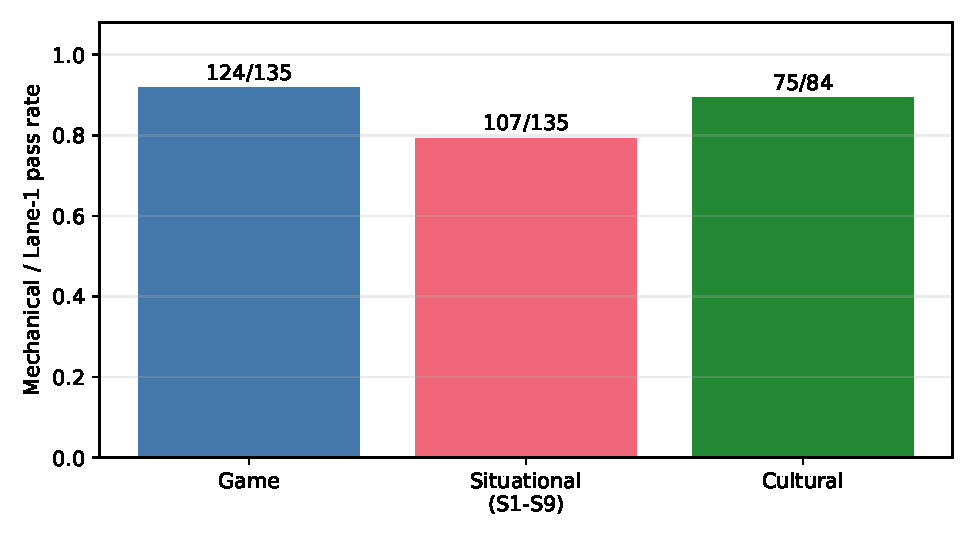
\includegraphics[width=\columnwidth]{fig/three_track_summary.pdf}
    \caption{Mechanical/Lane-1 pass rates for the completed subset of each track. Different formats and evaluators make these descriptive track summaries, not a controlled ranking of task difficulty.}
    \label{fig:three_tracks}
\end{figure}

Together, the three tracks contain 354 first-pass candidates over 32 distinct scenarios. Their evidence is intentionally asymmetric: games have formal references; cultural cases have reference-feature comparisons and expect/avoid criteria; situational cases have executable validation but neither a unique structural reference nor completed semantic annotations. We report unavailable cells rather than manufacture cross-track comparability.\todo{the last sentence is cryptic}

%\subsection
\paragraph{Game track: LLMs can construct mechanically valid POSGs}\todo{ideally, paragraph headings summarize the FINDING}
Across all trials, 124/135 (91.85\%) succeed on the first attempt. Recorded repair rounds produce a contract-valid final artifact for 135/135 trials. A separate post-hoc Lane-1 audit passes 134/135; the sole failure is DeepSeek G9 in run 1. These quantities answer different questions: first-pass validity measures unaided generation, repair-assisted validity measures the complete generation pipeline, and Lane 1 is a later stricter audit.

The evaluation flow is \emph{first response $\rightarrow$ optional logged repair $\rightarrow$ contract-valid final artifact $\rightarrow$ common post-hoc Lane 1 $\rightarrow$ structural comparison}. A repaired artifact is never counted as a first-pass success, and structural F1 is computed on the final artifact independently of its repair history.

\begin{table*}[t]
\centering
\small
\caption{Mechanical reliability over 27 trials per LLM. Brackets give descriptive 95\% Wilson intervals for first-pass proportions; trials span nine games and are not assumed to be IID population draws.}
\label{tab:main_results}
\begin{tabular}{lrrr}
\toprule
LLM & First pass & 95\% Wilson CI & Lane 1 \\
\midrule
Claude Opus 5 & 27/27 & [.875, 1.000] & 27/27 \\
DeepSeek V4 Flash & 23/27 & [.675, .941] & 26/27 \\
GPT-5.6 Sol & 26/27 & [.817, .993] & 27/27 \\
Llama 3.3 70B & 22/27 & [.633, .918] & 27/27 \\
Qwen 3.8 27B & 26/27 & [.817, .993] & 27/27 \\
\bottomrule
\end{tabular}
\end{table*}

\begin{table*}[t]
\centering
\small
\caption{Permutation-invariant structural comparison over 27 final artifacts per LLM. Means are supplemented by median and IQR; machine-readable results also report game-clustered bootstrap intervals.}
\label{tab:structural_results}
\begin{tabular}{lrrrrr}
\toprule
LLM & Coverage & Precision & Mean F1 & Median [Q1,Q3] & Exact \\
\midrule
Claude Opus 5 & .3133 & .1416 & .1709 & .1128 [.0597,.2312] & 1/27 \\
DeepSeek V4 Flash & .3255 & .2679 & .2696 & .1769 [.1171,.1941] & 4/27 \\
GPT-5.6 Sol & .5558 & .4879 & .4981 & .2500 [.1333,1.000] & 8/27 \\
Llama 3.3 70B & .5312 & .4528 & .4719 & .2000 [.1461,1.000] & 9/27 \\
Qwen 3.8 27B & .4324 & .4147 & .4087 & .1778 [.1524,.9441] & 6/27 \\
\bottomrule
\end{tabular}
\end{table*}

%\subsection
\emph{Lane 2: Structural fidelity conditional on validity\quad}
The stronger matcher materially changes the scale but strengthens rather than weakens the separation. Mean F1 is 0.3639 over all 135 final artifacts and 0.3660 among the 134 Lane-1 passes, versus 0.7178 under the old fallback. Among passing artifacts, median F1 is 0.1778, Q1--Q3 is [0.1258, 0.7396], and 28/134 score exactly 1. In descriptive threshold counts, 100/134 (74.63\%) fall below 0.75 and 33/134 (24.63\%) reach at least 0.90. These cutoffs summarize the distribution; they are not validated quality categories.

\begin{figure}[t]
    \centering
    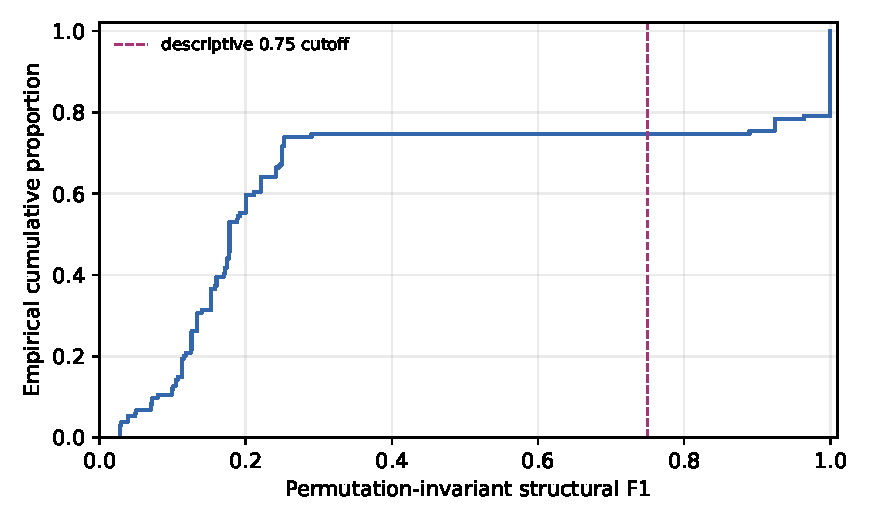
\includegraphics[width=\columnwidth]{fig/matched_f1_ecdf.pdf}
    \caption{ECDF of permutation-invariant structural F1 for the 134 Lane-1-passing game artifacts. The dashed 0.75 cutoff is descriptive, not a definition of fidelity.}
    \label{fig:matched_ecdf}
\end{figure}

Claude illustrates the separation particularly clearly: it succeeds on all 27 first passes and Lane-1 audits, yet mean matched precision is 0.1416 and mean F1 is 0.1709. Low precision means its artifacts contain additional matched structural mass relative to the compact references; it does not by itself prove those additions wrong. The inspected G6 example identifies one addition explicitly excluded by the case specification.

%\subsection
\emph{Structural failure case study\quad}\todo{I think this can go into the appendix}
\begin{figure}[t]
    \centering
    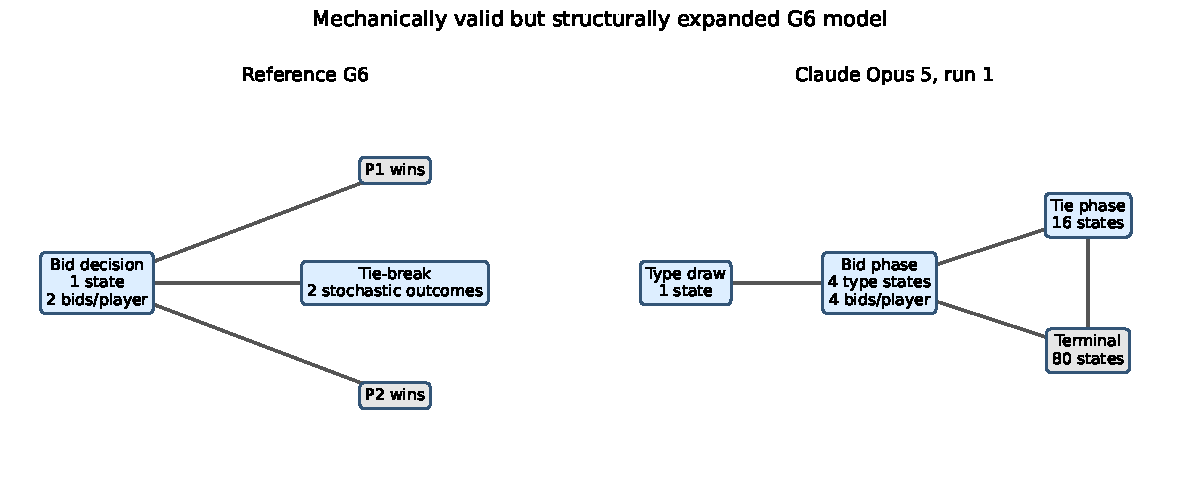
\includegraphics[width=\columnwidth]{fig/g6_claude_failure_case.pdf}
    \caption{Compressed phase graph for G6 versus the mechanically valid Claude Opus 5 artifact from run 1 (matched F1 0.0383). The candidate has 101 states. Unlike the two-bid-level reference, it introduces bids $\{0,1,2,3\}$ despite the rubric explicitly disallowing invented bid amounts, and expands the dynamics through four type states and 16 tie states. Nodes are grouped by verified phase prefix for legibility.}
    \label{fig:g6_failure}
\end{figure}
This is a confirmed unsupported expansion rather than merely a low score. Across all 107 non-exact artifacts, objective count-level flags include terminal-count mismatch in 99, additional states in 55, fewer states in 41, additional transition supports in 52, and stochastic-profile-rate mismatch in 41. Categories overlap. Except for inspected cases such as G6, these are structural differences requiring semantic inspection, not automatically errors.

%\subsection
\emph{Run-to-run stability within LLM--game pairs\quad}
For each of the 45 LLM--game pairs, we compute variation across its three observed generations. Overall mean within-pair F1 SD is 0.1679 and the median within-pair range is 0.0591. Only 4/45 pairs match the reference exactly in all three runs, while 15/45 generation triples are mutually structurally equivalent under all three pairwise matches. Qwen shows the largest observed variation (mean within-pair SD 0.3601; median range 0.7865), whereas GPT has the smallest (0.0618; median range 0). These are descriptive summaries of three generations, not stable variance estimates.

\begin{table}[t]
\centering\scriptsize
\caption{Within-pair structural variation across three generations. ``Equivalent'' counts triples whose three pairwise matched scores are 1.}
\label{tab:stability}
\begin{tabular}{lrrr}
\toprule
LLM & Mean SD & Median range & Equivalent \\
\midrule
Claude & .0715 & .0005 & 4/9 \\
DeepSeek & .1775 & .1053 & 1/9 \\
GPT & .0618 & .0000 & 5/9 \\
Llama & .1684 & .1184 & 4/9 \\
Qwen & .3601 & .7865 & 1/9 \\
\bottomrule
\end{tabular}
\end{table}

%\subsection
\emph{Reference complexity and fidelity\quad}
With only nine games, complexity analysis is exploratory. Across six pre-specified reference metrics, state count ($\rho=.053$), terminal count ($\rho=.053$), action profiles ($\rho=.202$), transition supports ($\rho=.009$), and average branching ($\rho=.053$) show little monotonic association with mean matched F1. The stochastic-profile fraction has $\rho=-.677$. Although its descriptive two-sided $p=.045$, the small case count and correlated metrics preclude confirmatory or causal interpretation; it is a hypothesis for a larger benchmark, not an established complexity law.

\begin{table}[t]
\centering
\small
\caption{Game-track reliability by repeated run. ``Final'' includes explicitly recorded repair rounds; attempts counts every first pass and repair call.}
\label{tab:game_runs}
\begin{tabular}{lrrr}
\toprule
Run & First-pass valid & Final valid & Attempts \\
\midrule
1 & 43/45 (95.56\%) & 45/45 & 47 \\
2 & 41/45 (91.11\%) & 45/45 & 50 \\
3 & 40/45 (88.89\%) & 45/45 & 68 \\
\midrule
All & 124/135 (91.85\%) & 135/135 & 165 \\
\bottomrule
\end{tabular}
\end{table}

%\subsection
\paragraph{Situational track: LLMs generate mostly executable Python POSGs}
Across the balanced S1--S9 subset, 114/135 first-pass programs execute, 110/135 pass the notebook's validation stage, and 107/135 pass the complete mechanical verdict. Claude and GPT each pass 27/27, Llama 20/27, Qwen 17/27, and DeepSeek 16/27. These rates come directly from saved notebook output rather than from the presence of source files. Repair files are retained but excluded from the headline. The spread is larger than in the game track, consistent with the situational cases' longer, less tightly specified dynamics, but the experiment does not isolate which property causes the difference.

\begin{table}[t]
\centering
\small
\caption{Situational S1--S9 first-pass funnel (three generations per LLM--case pair). S10--S11 are excluded because their saved execution log is incomplete.}
\label{tab:situational}
\begin{tabular}{lrrr}
\toprule
LLM & Executes & Validates & Mechanical pass \\
\midrule
Claude Opus 5 & 27/27 & 27/27 & 27/27 (100\%) \\
GPT-5.6 Sol & 27/27 & 27/27 & 27/27 (100\%) \\
Llama 3.3 70B & 25/27 & 22/27 & 20/27 (74.07\%) \\
Qwen 3.8 27B & 19/27 & 18/27 & 17/27 (62.96\%) \\
DeepSeek V4 Flash & 16/27 & 16/27 & 16/27 (59.26\%) \\
\midrule
All & 114/135 & 110/135 & 107/135 (79.26\%) \\
\bottomrule
\end{tabular}
\end{table}

The artifacts also contain generated source programs, but the completed experiment records no reference-backed graph comparison and no finished Lane-3 annotation set. Graph statistics computed from these programs would characterize generated topology, not measure fidelity. Consequently, this track contributes a defensible Lane-1 result but no Lane-2 or Lane-3 performance number.

%\subsection
\paragraph{Cultural track: LLM-generated POSGs mostly pass automated context/semantic diagnostics}
The cultural track has 84 candidates. Strict parsing succeeds for 52/84; documented fence/brace recovery produces parseable candidates for 82/84, and 75/84 pass Lane 1. By run, GPT and Claude each pass Lane 1 on all 28 candidates. Llama passes 8/14 anonymized and 11/14 country-named candidates. Across the 82 parseable candidates, mean fallback Lane-2 F1 is 0.5533. By LLM and condition it is 0.6386 vs 0.5777 for GPT, 0.6449 vs 0.6554 for Llama, and 0.4187 vs 0.3977 for Claude (anonymized vs location named).

For Lane 3, all 82 parseable candidates pass the automated expect/avoid checklist and their mean automated semantic score is 0.8963. Mean scores change by $-0.006$, $-0.007$, and $-0.001$ when location is revealed for GPT, Llama, and Claude respectively. These are descriptive diagnostics: providers differ for Llama across conditions, there is one sample per cell, reference wording differs slightly in six bullets, and no completed human study validates the automated semantic or bias checks. In particular, checklist passage is not proof of semantic faithfulness, and diagnostic bias flags are not evidence that a world model is biased.

%\subsection
\emph{Lane-3 evidence and its boundary\quad}
The game evaluator records 135/135 passes on its automated Lane-3 checklist, while the cultural evaluator records 82/84 (all parseable candidates) and mean automated semantic score 0.8963. These checks establish that the implemented criteria fired as recorded; they do not establish agreement with human judgment. The situational track has no completed Lane-3 result. Accordingly, our empirical claim is about available automated diagnostics, not human-validated semantic fidelity.

\begin{table*}[t]
\centering
\small
\caption{Cultural-track results by LLM and prompt condition (14 cases per row). ``Recovered'' denotes documented fence/brace recovery after strict parsing; semantic scores are automated diagnostics, not human judgments.}
\label{tab:cultural}
\begin{tabular}{llrrrrr}
\toprule
LLM & Condition & Strict & Recovered & Lane 1 & Structural F1 & Semantic \\
\midrule
GPT-5.6 Sol & Anonymized & 13/14 & 1 & 14/14 & .6386 & .9454 \\
GPT-5.6 Sol & Country named & 13/14 & 1 & 14/14 & .5777 & .9393 \\
Llama 3.3 70B & Anonymized & 0/14 & 12 & 8/14 & .6449 & .8380 \\
Llama 3.3 70B & Country named & 0/14 & 14 & 11/14 & .6554 & .8307 \\
Claude Opus 5 & Anonymized & 13/14 & 1 & 14/14 & .4187 & .9086 \\
Claude Opus 5 & Country named & 13/14 & 1 & 14/14 & .3977 & .9071 \\
\midrule
All & --- & 52/84 & 30 & 75/84 & --- & --- \\
\bottomrule
\end{tabular}
\end{table*}

\section{Discussion and Failure Analysis}
Mechanical correctness is necessary but insufficient for a trustworthy executable world model. In the game track nearly every artifact passes Lane 1, while permutation-invariant structural agreement spans a wide range. Restoring the intended matcher lowers rather than eliminates the observed gap, and the conditional result changes little when the sole Lane-1 failure is removed. Differences can reflect under-modeling, unsupported expansion, transition or terminal differences, or an alternative but valid granularity. The G6 audit confirms one unsupported invention, but we deliberately do not relabel every non-exact match as a semantic error.

This distinction matters conceptually for Physical AI even though the present cases are symbolic controls. An omitted successor can make a hazardous outcome appear unreachable; an invented reverse edge can make an irreversible action appear recoverable; wrong stochasticity changes risk estimates; a shortened horizon hides delayed consequences; and omitted or extra actions change estimated controllability. The experiments demonstrate the need for formal evaluation, not real-world safety. No downstream planner or controller is evaluated.

\section{Limitations}
The experiments use symbolic discrete POSGs rather than continuous perceptual or physical dynamics. The game study and reported situational subset have only three generations per LLM--case pair; the cultural track has one sample per condition. Provider/LLM versions may change, and Llama's cultural provider differs by condition. Exhaustive rollout and matching are bounded at depth three. The restored matcher is permutation-invariant under our tests but remains approximate, depends on finite-horizon conversion, and can penalize alternative valid granularity; its F1 is structural rather than semantic fidelity. The complexity analysis has only nine game units. Human Lane-3 validation is incomplete, so semantic scores and flags remain diagnostic. Situational S10--S11 are excluded because their execution record is incomplete, and the hand-authored v3 JSON track is not reported as LLM performance. We do not measure downstream planning, control, empowerment, reversibility, or real-world safety.

\section{Conclusion}
\label{sec:conclusion}
Across three empirical tracks we analyze 354 first-pass candidates: 135 reference-backed games, 135 logged situational Python POSGs, and 84 toy JSON world models. In games, repair makes all final artifacts available and 134 pass the common mechanical audit, but the restored permutation-invariant matcher yields mean F1 0.3660 among those passes and only 28 exact scores. Within-pair variation and the inspected G6 expansion show why aggregate executability cannot substitute for dynamics evaluation. Situational and cultural results retain their different evidence boundaries. Executability is therefore a gate, not evidence of structural fidelity. Future work should add embodied dynamics, complete human semantic annotation, test matching across valid granularities, and evaluate downstream policies.


% \section{References}
% \label{sec:references}

% Papers to be submitted to NeurIPS 2026 must be prepared according to the
% instructions presented here. Papers may only be up to {\bf nine} pages long, including figures. \textbf{Papers that exceed the page limit will not be reviewed (or in any other way considered) for presentation at the conference.}
% Additional pages \emph{containing acknowledgments, references, checklist, and optional technical appendices} do not count as content pages. 


% The margins in 2026 are the same as those in previous years.


% Authors are required to use the NeurIPS \LaTeX{} style files obtainable at the NeurIPS website as indicated below. Please make sure you use the current files and not previous versions. Tweaking the style files may be grounds for desk rejection.


% \subsection{Retrieval of style files}


% The style files for NeurIPS and other conference information are available on the website at
% \begin{center}
%   \url{https://neurips.cc}.
% \end{center}
% % The file \verb+neurips_2026.pdf+ contains these instructions and illustrates the various formatting requirements your NeurIPS paper must satisfy.


% The only supported style file for NeurIPS 2026 is \verb+neurips_2026.sty+, rewritten for \LaTeXe{}. \textbf{Previous style files for \LaTeX{} 2.09,  Microsoft Word, and RTF are no longer supported.}


% The \LaTeX{} style file contains three optional arguments: 
% \begin{itemize}
% \item \verb+final+, which creates a camera-ready copy, 
% \item \verb+preprint+, which creates a preprint for submission to, e.g., arXiv, \item \verb+nonatbib+, which will not load the \verb+natbib+ package for you in case of package clash.
% \end{itemize}


% \paragraph{Preprint option}
% If you wish to post a preprint of your work online, e.g., on arXiv, using the NeurIPS style, please use the \verb+preprint+ option. This will create a nonanonymized version of your work with the text ``Preprint. Work in progress.'' in the footer. This version may be distributed as you see fit, as long as you do not say which conference it was submitted to. Please \textbf{do not} use the \verb+final+ option, which should \textbf{only} be used for papers accepted to NeurIPS.


% At submission time, please omit the \verb+final+ and \verb+preprint+ options. This will anonymize your submission and add line numbers to aid review. Please do \emph{not} refer to these line numbers in your paper as they will be removed during generation of camera-ready copies.


% The file \verb+neurips_2026.tex+ may be used as a ``shell'' for writing your paper. All you have to do is replace the author, title, abstract, and text of the paper with your own.


% The formatting instructions contained in these style files are summarized in Sections \ref{gen_inst}, \ref{headings}, and \ref{others} below.


% \section{General formatting instructions}
% \label{gen_inst}


% The text must be confined within a rectangle 5.5~inches (33~picas) wide and
% 9~inches (54~picas) long. The left margin is 1.5~inch (9~picas).  Use 10~point
% type with a vertical spacing (leading) of 11~points.  Times New Roman is the
% preferred typeface throughout, and will be selected for you by default.
% Paragraphs are separated by \nicefrac{1}{2}~line space (5.5 points), with no
% indentation.


% The paper title should be 17~point, initial caps/lower case, bold, centered
% between two horizontal rules. The top rule should be 4~points thick and the
% bottom rule should be 1~point thick. Allow \nicefrac{1}{4}~inch space above and
% below the title to rules. All pages should start at 1~inch (6~picas) from the
% top of the page.


% For the final version, authors' names are set in boldface, and each name is
% centered above the corresponding address. The lead author's name is to be listed
% first (left-most), and the co-authors' names (if different address) are set to
% follow. If there is only one co-author, list both author and co-author side by
% side.


% Please pay special attention to the instructions in Section \ref{others}
% regarding figures, tables, acknowledgments, and references.

% \section{Headings: first level}
% \label{headings}


% All headings should be lower case (except for first word and proper nouns),
% flush left, and bold.


% First-level headings should be in 12-point type.


% \subsection{Headings: second level}


% Second-level headings should be in 10-point type.


% \subsubsection{Headings: third level}


% Third-level headings should be in 10-point type.


% \paragraph{Paragraphs}


% There is also a \verb+\paragraph+ command available, which sets the heading in
% bold, flush left, and inline with the text, with the heading followed by 1\,em
% of space.


% \section{Citations, figures, tables, references}
% \label{others}


% These instructions apply to everyone.


% \subsection{Citations within the text}


% The \verb+natbib+ package will be loaded for you by default.  Citations may be
% author/year or numeric, as long as you maintain internal consistency.  As to the
% format of the references themselves, any style is acceptable as long as it is
% used consistently.


% The documentation for \verb+natbib+ may be found at
% \begin{center}
%   \url{http://mirrors.ctan.org/macros/latex/contrib/natbib/natnotes.pdf}
% \end{center}
% Of note is the command \verb+\citet+, which produces citations appropriate for
% use in inline text.  For example,
% \begin{verbatim}
%    \citet{hasselmo} investigated\dots
% \end{verbatim}
% produces
% \begin{quote}
%   Hasselmo, et al.\ (1995) investigated\dots
% \end{quote}


% If you wish to load the \verb+natbib+ package with options, you may add the
% following before loading the \verb+neurips_2026+ package:
% \begin{verbatim}
%    \PassOptionsToPackage{options}{natbib}
% \end{verbatim}


% If \verb+natbib+ clashes with another package you load, you can add the optional
% argument \verb+nonatbib+ when loading the style file:
% \begin{verbatim}
%    \usepackage[nonatbib]{neurips_2026}
% \end{verbatim}


% As submission is double blind, refer to your own published work in the third
% person. That is, use ``In the previous work of Jones et al.\ [4],'' not ``In our
% previous work [4].'' If you cite your other papers that are not widely available
% (e.g., a journal paper under review), use anonymous author names in the
% citation, e.g., an author of the form ``A.\ Anonymous'' and include a copy of the anonymized paper in the supplementary material.


% \subsection{Footnotes}


% Footnotes should be used sparingly.  If you do require a footnote, indicate
% footnotes with a number\footnote{Sample of the first footnote.} in the
% text. Place the footnotes at the bottom of the page on which they appear.
% Precede the footnote with a horizontal rule of 2~inches (12~picas).


% Note that footnotes are properly typeset \emph{after} punctuation
% marks.\footnote{As in this example.}


% \subsection{Figures}


% \begin{figure}
%   \centering
%   \fbox{\rule[-.5cm]{0cm}{4cm} \rule[-.5cm]{4cm}{0cm}}
%   \caption{Sample figure caption. Explain what the figure shows and add a key take-away message to the caption.}
% \end{figure}


% All artwork must be neat, clean, and legible. Lines should be dark enough for
%  reproduction purposes. The figure number and caption always appear after the
% figure. Place one line space before the figure caption and one line space after
% the figure. The figure caption should be lower case (except for the first word and proper nouns); figures are numbered consecutively.


% You may use color figures.  However, it is best for the figure captions and the
% paper body to be legible if the paper is printed in either black/white or in
% color.


% \subsection{Tables}


% All tables must be centered, neat, clean, and legible.  The table number and
% title always appear before the table.  See Table~\ref{sample-table}.


% Place one line space before the table title, one line space after the
% table title, and one line space after the table. The table title must
% be lower case (except for the first word and proper nouns); tables are
% numbered consecutively.


% Note that publication-quality tables \emph{do not contain vertical rules}. We
% strongly suggest the use of the \verb+booktabs+ package, which allows for
% typesetting high-quality, professional tables:
% \begin{center}
%   \url{https://www.ctan.org/pkg/booktabs}
% \end{center}
% This package was used to typeset Table~\ref{sample-table}.


% \begin{table}
%   \caption{Sample table caption. Explain what the table shows and add a key take-away message to the caption.}
%   \label{sample-table}
%   \centering
%   \begin{tabular}{lll}
%     \toprule
%     \multicolumn{2}{c}{Part}                   \\
%     \cmidrule(r){1-2}
%     Name     & Description     & Size ($\mu$m) \\
%     \midrule
%     Dendrite & Input terminal  & $\approx$100     \\
%     Axon     & Output terminal & $\approx$10      \\
%     Soma     & Cell body       & up to $10^6$  \\
%     \bottomrule
%   \end{tabular}
% \end{table}

% \subsection{Math}
% Note that display math in bare TeX commands will not create correct line numbers for submission. Please use LaTeX (or AMSTeX) commands for unnumbered display math. (You really shouldn't be using \$\$ anyway; see \url{https://tex.stackexchange.com/questions/503/why-is-preferable-to} and \url{https://tex.stackexchange.com/questions/40492/what-are-the-differences-between-align-equation-and-displaymath} for more information.)

% \subsection{Final instructions}

% Do not change any aspects of the formatting parameters in the style files.  In
% particular, do not modify the width or length of the rectangle the text should
% fit into, and do not change font sizes. Please note that pages should be
% numbered.


% \section{Preparing PDF files}


% Please prepare submission files with paper size ``US Letter,'' and not, for
% example, ``A4.''


% Fonts were the main cause of problems in the past years. Your PDF file must only
% contain Type 1 or Embedded TrueType fonts. Here are a few instructions to
% achieve this.


% \begin{itemize}


% \item You should directly generate PDF files using \verb+pdflatex+.


% \item You can check which fonts a PDF files uses.  In Acrobat Reader, select the
%   menu Files$>$Document Properties$>$Fonts and select Show All Fonts. You can
%   also use the program \verb+pdffonts+ which comes with \verb+xpdf+ and is
%   available out-of-the-box on most Linux machines.


% \item \verb+xfig+ ``patterned'' shapes are implemented with bitmap fonts.  Use
%   "solid" shapes instead.


% \item The \verb+\bbold+ package almost always uses bitmap fonts.  You should use
%   the equivalent AMS Fonts:
% \begin{verbatim}
%    \usepackage{amsfonts}
% \end{verbatim}
% followed by, e.g., \verb+\mathbb{R}+, \verb+\mathbb{N}+, or \verb+\mathbb{C}+
% for $\mathbb{R}$, $\mathbb{N}$ or $\mathbb{C}$.  You can also use the following
% workaround for reals, natural and complex:
% \begin{verbatim}
%    \newcommand{\RR}{I\!\!R} %real numbers
%    \newcommand{\Nat}{I\!\!N} %natural numbers
%    \newcommand{\CC}{I\!\!\!\!C} %complex numbers
% \end{verbatim}
% Note that \verb+amsfonts+ is automatically loaded by the \verb+amssymb+ package.


% \end{itemize}


% If your file contains type 3 fonts or non embedded TrueType fonts, we will ask
% you to fix it.


% \subsection{Margins in \LaTeX{}}


% Most of the margin problems come from figures positioned by hand using
% \verb+\special+ or other commands. We suggest using the command
% \verb+\includegraphics+ from the \verb+graphicx+ package. Always specify the
% figure width as a multiple of the line width as in the example below:
% \begin{verbatim}
%    \usepackage[pdftex]{graphicx} ...
%    \includegraphics[width=0.8\linewidth]{myfile.pdf}
% \end{verbatim}
% See Section 4.4 in the graphics bundle documentation
% (\url{http://mirrors.ctan.org/macros/latex/required/graphics/grfguide.pdf})


% A number of width problems arise when \LaTeX{} cannot properly hyphenate a
% line. Please give LaTeX hyphenation hints using the \verb+\-+ command when
% necessary.

% \begin{ack}
% Use unnumbered first level headings for the acknowledgments. All acknowledgments
% go at the end of the paper before the list of references. Moreover, you are required to declare
% funding (financial activities supporting the submitted work) and competing interests (related financial activities outside the submitted work).
% More information about this disclosure can be found at: \url{https://neurips.cc/Conferences/2026/PaperInformation/FundingDisclosure}.


% Do {\bf not} include this section in the anonymized submission, only in the final paper. You can use the \texttt{ack} environment provided in the style file to automatically hide this section in the anonymized submission.
% \end{ack}

%\section*{References}
%\bibliographystyle{plainnat}
\bibliographystyle{unsrtnat} 
%\bibliography{reference}

%References follow the acknowledgments in the camera-ready paper. Use unnumbered first-level heading for
%the references. Any choice of citation style is acceptable as long as you are
%consistent. It is permissible to reduce the font size to \verb+small+ (9 point)
%when listing the references.
%Note that the Reference section does not count towards the page limit.
\medskip


{
\small
\bibliography{reference}

%[1] Alexander, J.A.\ \& Mozer, M.C.\ (1995) Template-based algorithms for connectionist rule extraction. In G.\ Tesauro, D.S.\ Touretzky and T.K.\ Leen (eds.), {\it Advances in Neural Information Processing Systems 7}, pp.\ 609--616. Cambridge, MA: MIT Press.


%[2] Bower, J.M.\ \& Beeman, D.\ (1995) {\it The Book of GENESIS: Exploring Realistic Neural Models with the GEneral NEural SImulation System.}  New York: TELOS/Springer--Verlag.


%[3] Hasselmo, M.E., Schnell, E.\ \& Barkai, E.\ (1995) Dynamics of learning and recall at excitatory recurrent synapses and cholinergic modulation in rat hippocampal region CA3. {\it Journal of Neuroscience} {\bf 15}(7):5249-5262.
}


%%%%%%%%%%%%%%%%%%%%%%%%%%%%%%%%%%%%%%%%%%%%%%%%%%%%%%%%%%%%

\newpage
\appendix

\section{Additional graph diagnostics}
\subsection{Case-level results}
\begin{table}[t]
\centering
\small
\caption{Game results by case, pooled over five LLMs and three runs (15 candidates per case). F1 uses permutation-invariant matching.}
\label{tab:game_cases}
\begin{tabular}{lrrrrrrrrr}
\toprule
Case & G1 & G2 & G3 & G4 & G5 & G6 & G7 & G8 & G9 \\
\midrule
Lane 1 & 15 & 15 & 15 & 15 & 15 & 15 & 15 & 15 & 14 \\
Mean F1 & .345 & .095 & .321 & .634 & .468 & .183 & .610 & .492 & .127 \\
\bottomrule
\end{tabular}
\end{table}

\begin{table}[t]
\centering
\small
\caption{Situational first-pass mechanical validity by case, pooled over five LLMs and three generations (15 attempts per case).}
\label{tab:situational_cases}
\begin{tabular}{lrrrrrrrrr}
\toprule
Case & S1 & S2 & S3 & S4 & S5 & S6 & S7 & S8 & S9 \\
\midrule
Pass & 13 & 13 & 11 & 10 & 13 & 11 & 12 & 13 & 11 \\
Total & 15 & 15 & 15 & 15 & 15 & 15 & 15 & 15 & 15 \\
\bottomrule
\end{tabular}
\end{table}

\begin{table*}[t]
\centering
\small
\caption{Cultural results by case, pooled over three LLMs and two prompt conditions (six candidates per case). Semantic values are automated diagnostics.}
\label{tab:cultural_cases}
\begin{tabular}{lrrrrrrrrrrrrrr}
\toprule
Case & C1 & C2 & C3 & C4 & C5 & C6 & C7 & C8 & C9 & C10 & C11 & C12 & C13 & C14 \\
\midrule
Lane 1 & 6 & 6 & 6 & 6 & 5 & 6 & 4 & 6 & 5 & 5 & 4 & 4 & 6 & 6 \\
Mean F1 & .676 & .634 & .630 & .595 & .528 & .411 & .377 & .529 & .524 & .546 & .490 & .647 & .461 & .692 \\
Mean semantic & .903 & .909 & .841 & .887 & .963 & .855 & .878 & .856 & .924 & .869 & .898 & .906 & .927 & .938 \\
\bottomrule
\end{tabular}
\end{table*}

Figure~\ref{fig:reference_comparison} characterizes the structural diversity of the nine reference games used by the evaluation. Figure~\ref{fig:qwen_example} records an earlier local-Qwen G1 artifact that passed structural rollout but failed game-specific reward and observation checks. This example is diagnostic and is not pooled with the five-LLM study.

\begin{figure}[t]
    \centering
    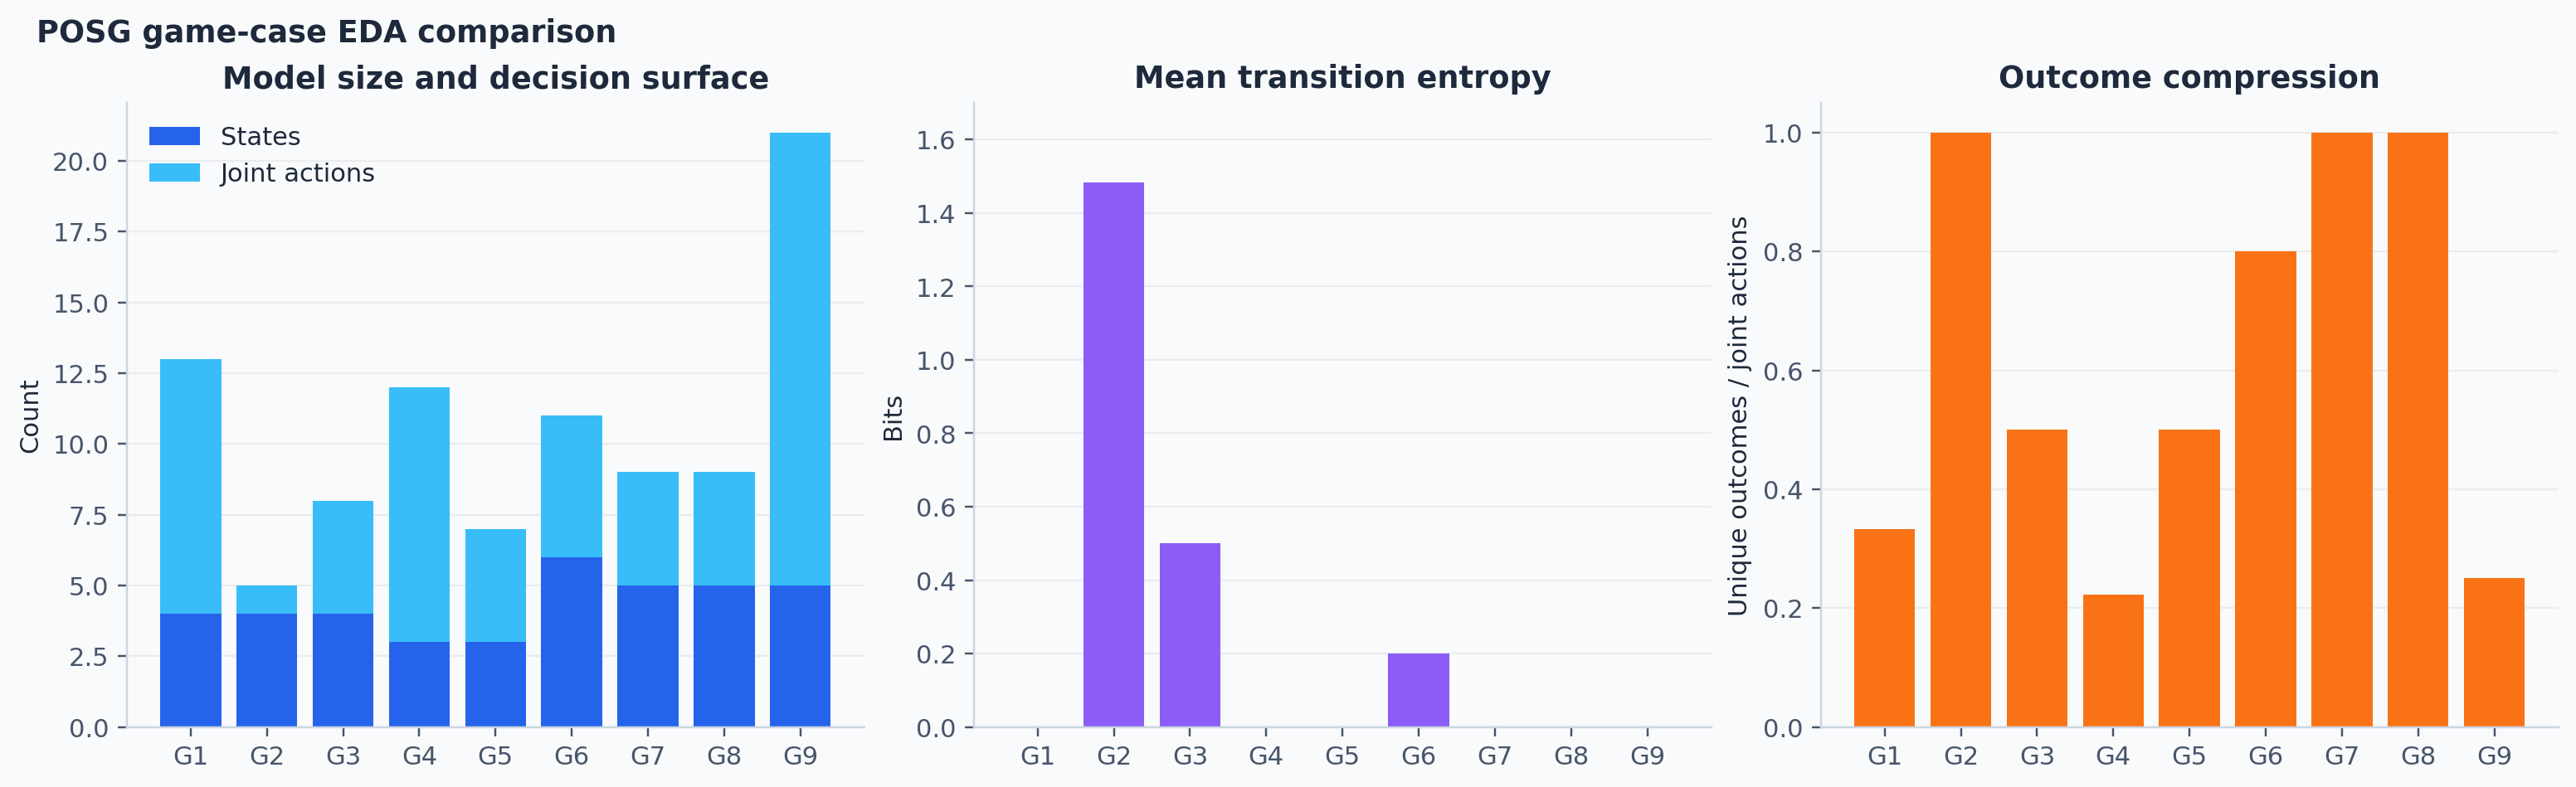
\includegraphics[width=\linewidth]{fig/game_case_comparison.png}
    \caption{Cross-case graph statistics for the G1--G9 reference fixtures. These are controls, not generated world model performance.}
    \label{fig:reference_comparison}
\end{figure}

\begin{figure}[t]
    \centering
    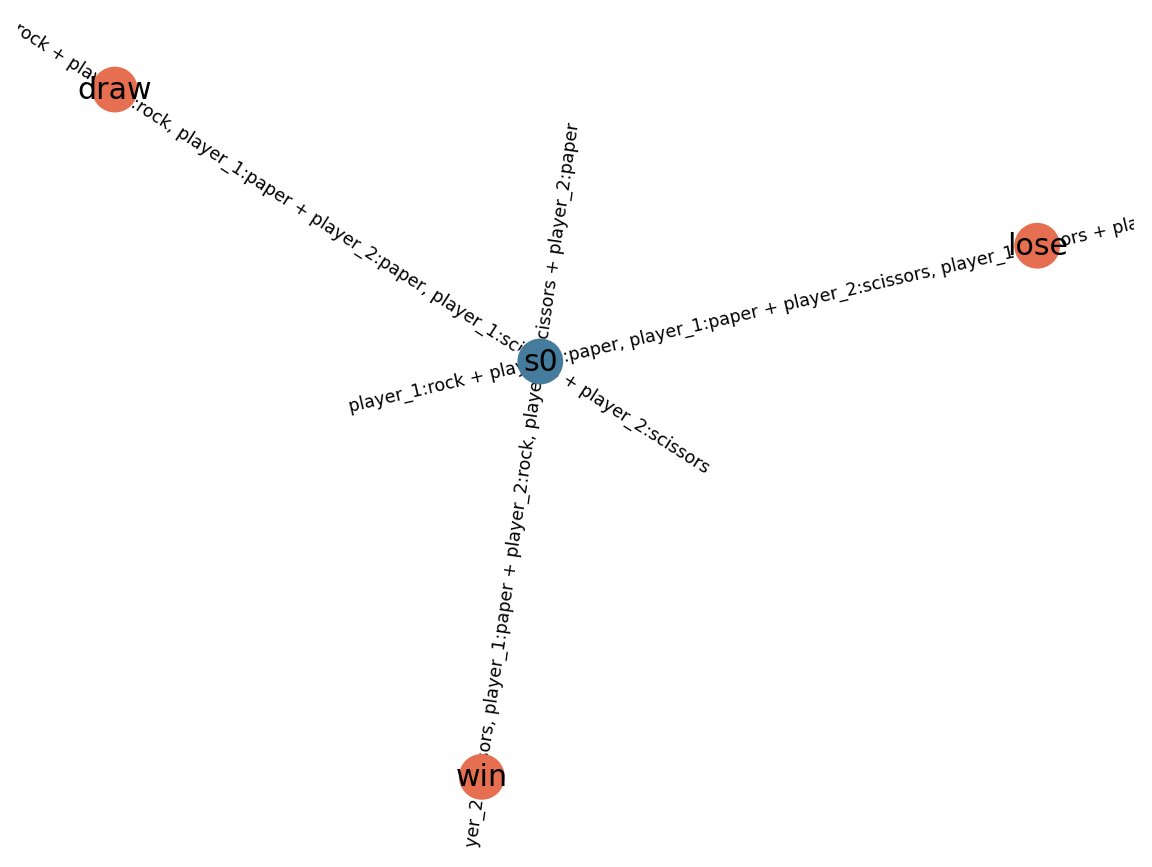
\includegraphics[width=.75\linewidth]{fig/qwen_g1_sample_003_graph.png}
    \caption{State graph for an earlier local-Qwen G1 sample. A plausible graph did not prevent incorrect rewards and player-specific observations, illustrating why topology alone is insufficient.}
    \label{fig:qwen_example}
\end{figure}

%%%%%%%%%%%%%%%%%%%%%%%%%%%%%%%%%%%%%%%%%%%%%%%%%%%%%%%%%%%%

% \todo[inline]{
% }
\section{Complete per-track results}
\label{app:full_tables}
The main text aggregates each track into a handful of numbers. Those aggregates carry the argument, but they hide the cells that compose them. We therefore report every per-case result here, and we draw out what the full tables show that the summaries cannot. Throughout, Lane~1 is the mechanical-validity audit, Lane~2 the structural comparison under the documented \texttt{feature\_multiset\_fallback} backend, and Lane~3 the automated expect/avoid checklist. The fallback backend is not an optimal graph matcher. We thus treat Lane-2 scores as comparable within a track, never as upper bounds on structural agreement.

\subsection{Toy track (T1.1--T4.4, JSON track)}
The toy track tests the evaluator, not the world models: its candidates are hand-authored zero-shot-v3 world models, so a well-behaved pipeline should award near-perfect scores. It largely does. We find that all ten cases pass the mechanical, checklist, and bias gates, and eight of ten recover the reference structure exactly under Lane~2 (Figure~\ref{fig:toy_comb}).

The three exceptions teach us more than the seven matches. Consider T2.2. It scores the lowest combined F1 (0.68) yet a precision of 0.94. The candidate misses almost nothing; it simply branches further than the reference. We observe the same coverage-driven pattern on T2.1 and T3.2. This is the granularity ambiguity of Section~\ref{sec:results} materialized in a setting where ground truth is unambiguous. We conclude that the evaluator penalizes finer modelling even when no reference structure is lost --- and that this coverage--precision asymmetry, not noise, is what dominates the LLM-generated tracks.


\begin{table}[t]
\centering
\small
\caption{Toy-track results (one hand-authored candidate per case). ``comb'' is Lane-2 combined F1; Lane 1, Lane 3, bias-free and overall are pass/fail.}
\label{tab:toy_full}
\begin{tabular}{lrrrrrrr}
\toprule
Case & Lane 1 & L2 cov & L2 prec & L2 comb & Lane 3 & Bias-free & Overall \\
\midrule
T1.1 & Pass & 1.00 & 1.00 & 1.00 & Pass & Pass & Pass \\
T1.2 & Pass & 1.00 & 1.00 & 1.00 & Pass & Pass & Pass \\
T2.1 & Pass & 0.69 & 0.90 & 0.78 & Pass & Pass & Pass \\
T2.2 & Pass & 0.53 & 0.94 & 0.68 & Pass & Pass & Pass \\
T3.1 & Pass & 1.00 & 1.00 & 1.00 & Pass & Pass & Pass \\
T3.2 & Pass & 0.65 & 0.88 & 0.75 & Pass & Pass & Pass \\
T4.1 & Pass & 1.00 & 1.00 & 1.00 & Pass & Pass & Pass \\
T4.2 & Pass & 1.00 & 1.00 & 1.00 & Pass & Pass & Pass \\
T4.3 & Pass & 1.00 & 0.92 & 0.96 & Pass & Pass & Pass \\
T4.4 & Pass & 1.00 & 1.00 & 1.00 & Pass & Pass & Pass \\
\bottomrule
\end{tabular}
\end{table}

\begin{figure}[t]
    \centering
    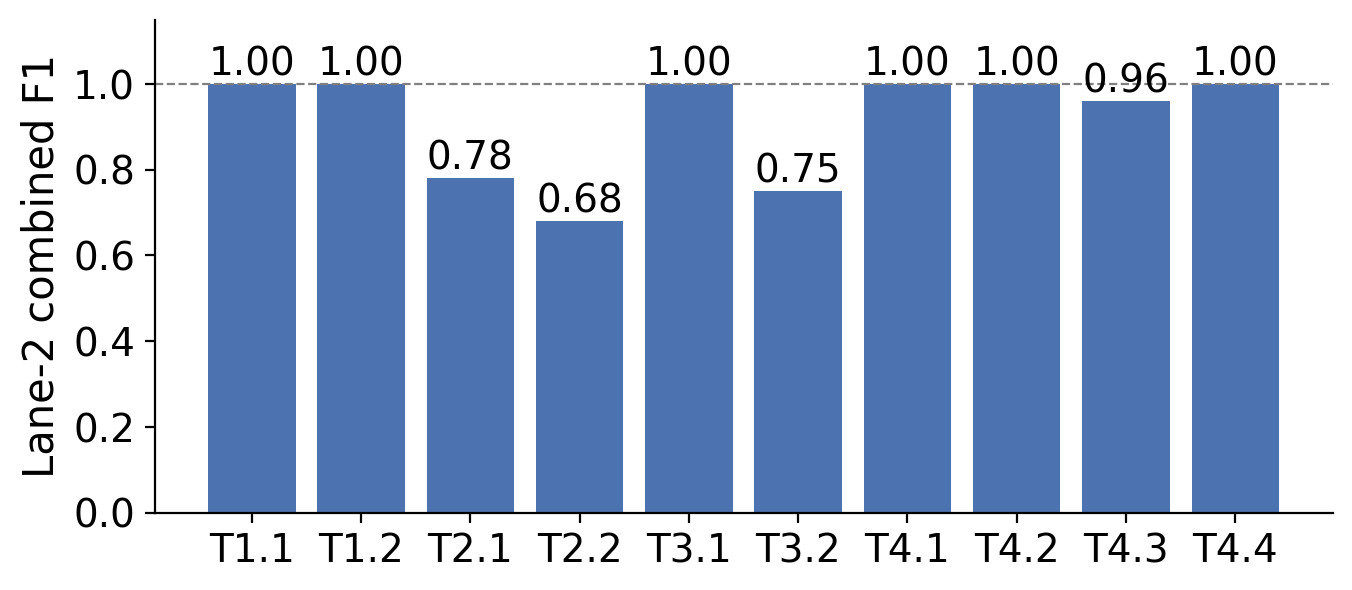
\includegraphics[width=.85\linewidth]{fig/toy_comb_f1.png}
    \caption{Lane-2 combined F1 across the toy-track cases. Structural agreement is exact on eight of ten cases and degrades only where candidates branch more finely than the reference, with coverage rather than precision accounting for the loss.}
    \label{fig:toy_comb}
\end{figure}

\subsection{Game track (G1--G9)}
Mechanical validity saturates in the game track; structural agreement does not. That contrast is the paper's thesis, and the per-case matrix in Table~\ref{tab:game_matrix} is where it becomes visible. We evaluate 135 candidates and find that 134 pass the mechanical audit and all 135 pass the checklist; the single Lane-1 failure belongs to DeepSeek on G9. At the per-cell level, as in the aggregate, executability is a solved gate.

Structure behaves differently. We establish three findings from the full matrix. First, case identity, not LLM identity, drives structural agreement: the within-LLM spread across cases (GPT-5.6 alone spans 0.21 to 1.00) dwarfs the between-LLM spread on any single case. Second, G2 and G6 depress every LLM simultaneously (0.10--0.36 and 0.11--0.74). When five independently prompted LLMs fail on the same fixture, we attribute the failure to the reference --- most plausibly its stochastic structure or terminal-state layout --- rather than to any LLM. Third, the LLMs separate even where coverage does not. Claude Opus 5 holds the second-highest coverage (0.91) yet the lowest combined F1 (0.52); its candidates recover most reference transitions but systematically add structure the reference lacks. Figures~\ref{fig:game_per_LLM} and \ref{fig:game_matrix_fig} display both views.

Finally, we note what does not happen: the bias gate never fires. All 135 candidates defer norm-relevant decisions to game-defined authorities. We report this as pipeline behavior, not as evidence about LLM safety.


\begin{table}[t]
\centering
\small
\caption{Game-track per-LLM aggregates (means over 9 cases $\times$ 3 runs; 27 candidates per LLM).}
\label{tab:game_full}
\begin{tabular}{lrrrrrrr}
\toprule
LLM & Cand. & Lane 1 & L2 cov & L2 comb & Lane 3 & Bias-free & Overall \\
\midrule
GPT-5.6 Sol & 27 & 27/27 & 0.94 & 0.79 & 27/27 & 27/27 & 27/27 \\
Claude Opus 5 & 27 & 27/27 & 0.91 & 0.52 & 27/27 & 27/27 & 27/27 \\
Llama 3.3 70B & 27 & 27/27 & 0.89 & 0.75 & 27/27 & 27/27 & 27/27 \\
Qwen 3.8 27B & 27 & 27/27 & 0.86 & 0.82 & 27/27 & 27/27 & 27/27 \\
DeepSeek V4 Flash & 27 & 26/27 & 0.78 & 0.71 & 27/27 & 27/27 & 26/27 \\
\bottomrule
\end{tabular}
\end{table}

\begin{figure}[t]
    \centering
    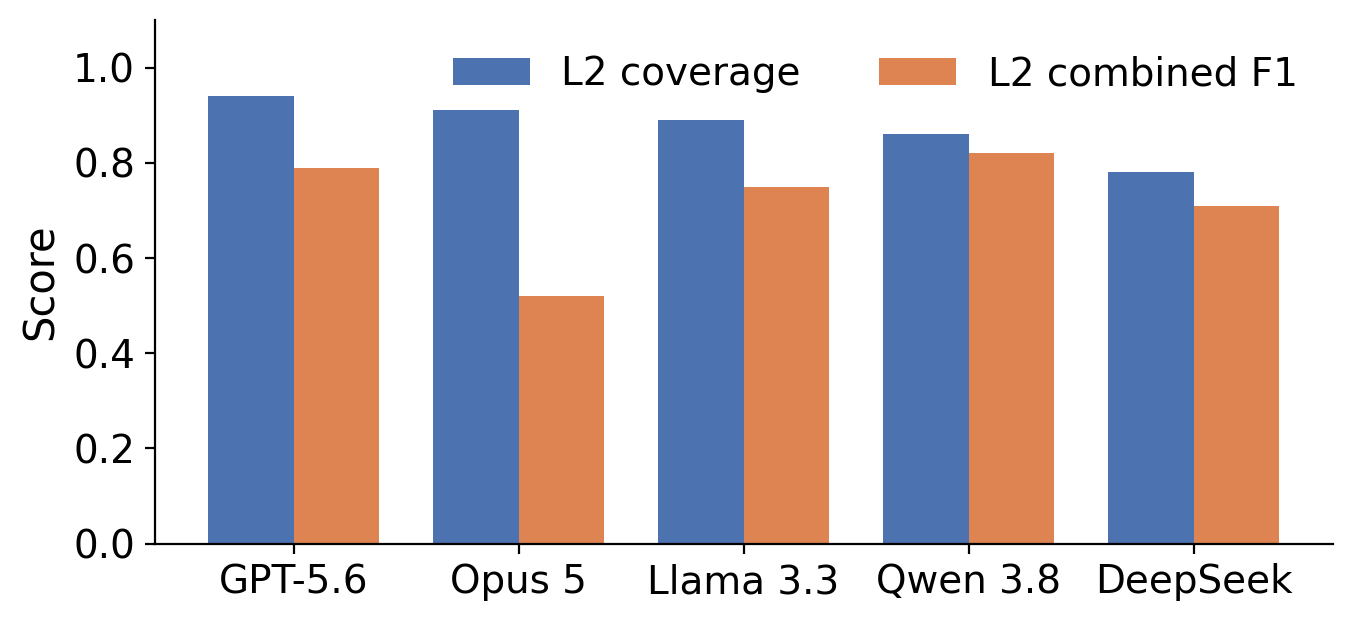
\includegraphics[width=.85\linewidth]{fig/game_per_model.png}
    \caption{Per-LLM Lane-2 coverage and combined F1 in the game track. Coverage remains near ceiling for every LLM, whereas combined F1 separates the LLMs, most visibly Claude Opus 5.}
    \label{fig:game_per_LLM}
\end{figure}

\begin{table*}[t]
\centering
\footnotesize
\caption{Game-track per-case breakdown showing Lane-2 Coverage / Combined $F_1$ (means over 3 runs). All cells achieve $3/3$ on Lane 1, Lane 3, and Bias-free, except DeepSeek on G9 ($2/3$ on Lane 1).}
\setlength{\tabcolsep}{4 pt}
\label{tab:game_matrix_full_compact}
\begin{tabular}{l *{9}{c}}
\toprule
LLM & G1 & G2 & G3 & G4 & G5 & G6 & G7 & G8 & G9 \\
\midrule
GPT-5.6 Sol       & .94 / .82 & .95 / .21 & .80 / .82 & 1.0 / 1.0 & .95 / .97 & .90 / .28 & 1.0 / 1.0 & 1.0 / 1.0 & .95 / .97 \\
Claude Opus 5     & 1.0 / .79 & .74 / .10 & .92 / .69 & .90 / .46 & 1.0 / .87 & .96 / .11 & .88 / .62 & .77 / .35 & 1.0 / .68 \\
Llama 3.3 70B     & .94 / .89 & .81 / .36 & .88 / .79 & 1.0 / 1.0 & .90 / .71 & .82 / .72 & 1.0 / 1.0 & .65 / .59 & 1.0 / .68 \\
Qwen 3.8 27B      & .88 / .93 & .91 / .18 & .87 / .88 & .93 / .96 & .90 / .95 & .64 / .74 & .77 / .86 & .88 / .93 & .93 / .96 \\
DeepSeek V4 Flash & .82 / .82 & .63 / .15 & .71 / .61 & .97 / .98 & .90 / .95 & .63 / .39 & .65 / .79 & .77 / .86 & .93 / .81$^\dagger$ \\
\bottomrule
\multicolumn{10}{l}{\footnotesize Values formatted as \textit{Coverage / Combined $F_1$}. $^\dagger$DeepSeek recorded a single Lane-1 failure on G9 (2/3).}
\end{tabular}
\end{table*}
\begin{figure*}[p]
    \centering
    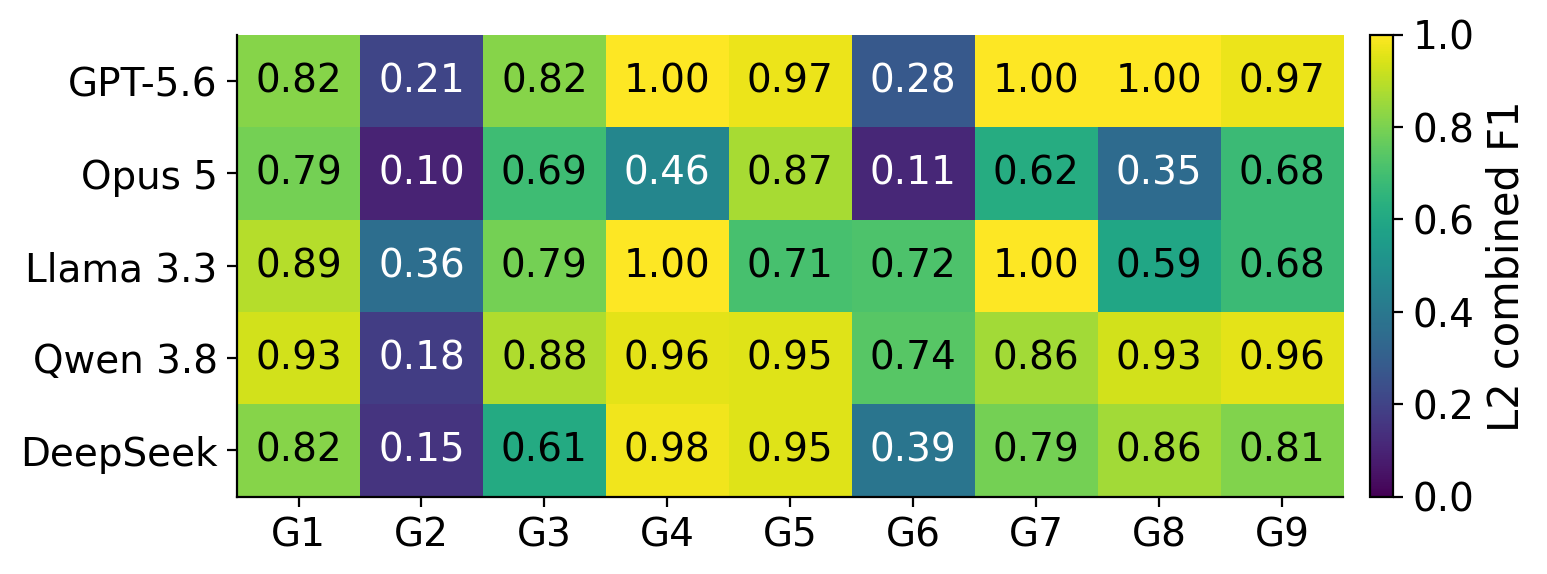
\includegraphics[width=.95\textwidth]{fig/game_model_case_heatmap.png}
    \caption{Lane-2 combined F1 by LLM and case in the game track. G2 and G6 depress every LLM simultaneously, suggesting reference properties that all candidates systematically miss rather than LLM-specific weaknesses.}
    \label{fig:game_matrix_fig}
\end{figure*}

\subsection{Situational track (S1--S11, Python POSG track)}
The situational track records execution artifacts, not scores. We can therefore measure generation behavior here, not fidelity --- and we read the artifact inventory in Table~\ref{tab:situational_full} accordingly.

The counts split the panel into two regimes, and the split is stark. GPT-5.6 and Claude Opus 5 sit at the three-attempt baseline nearly everywhere; Claude's only deviation is a single lost artifact on S10. Their first-pass programs execute and validate without repair. Qwen and DeepSeek behave oppositely. They accumulate surplus artifacts on the same cases --- eight apiece on S3, with DeepSeek also stacking retries on S4, S6, and S7. We find it consistent that precisely the two LLMs with the weakest mechanical pass rates in the balanced S1--S9 subset (Table~\ref{tab:situational}) carry the heaviest retry pressure (Figure~\ref{fig:situational_artifacts}). Repair loops absorb their generation budget. Still, we state the boundary plainly: artifact counts measure effort, never quality. This track contributes a Lane-1 result and nothing more.


\begin{table}[t]
\centering
\small
\caption{Situational-track artifacts per (LLM, case): preserved Python world model files per cell (base attempts g0--g2 plus retries).}
\label{tab:situational_full}
\begin{tabular}{lrrrrrrrrrrrrr}
\toprule
LLM & S1 & S2 & S3 & S4 & S5 & S6 & S7 & S8 & S9 & S10 & S11 & Cov. & Art. \\
\midrule
GPT-5.6 Sol & 3 & 3 & 3 & 3 & 3 & 3 & 3 & 3 & 3 & 3 & 3 & 11/11 & 33 \\
Claude Opus 5 & 3 & 3 & 3 & 3 & 3 & 3 & 3 & 3 & 3 & 2 & 3 & 11/11 & 32 \\
Llama 3.3 70B & 3 & 3 & 3 & 6 & 4 & 4 & 4 & 3 & 5 & 3 & 6 & 11/11 & 44 \\
Qwen 3.8 27B & 5 & 5 & 8 & 7 & 3 & 6 & 3 & 5 & 5 & 3 & 5 & 11/11 & 55 \\
DeepSeek V4 Flash & 4 & 3 & 8 & 4 & 4 & 5 & 6 & 4 & 4 & 6 & 5 & 11/11 & 53 \\
\bottomrule
\end{tabular}
\end{table}

\begin{figure*}[p]
    \centering
    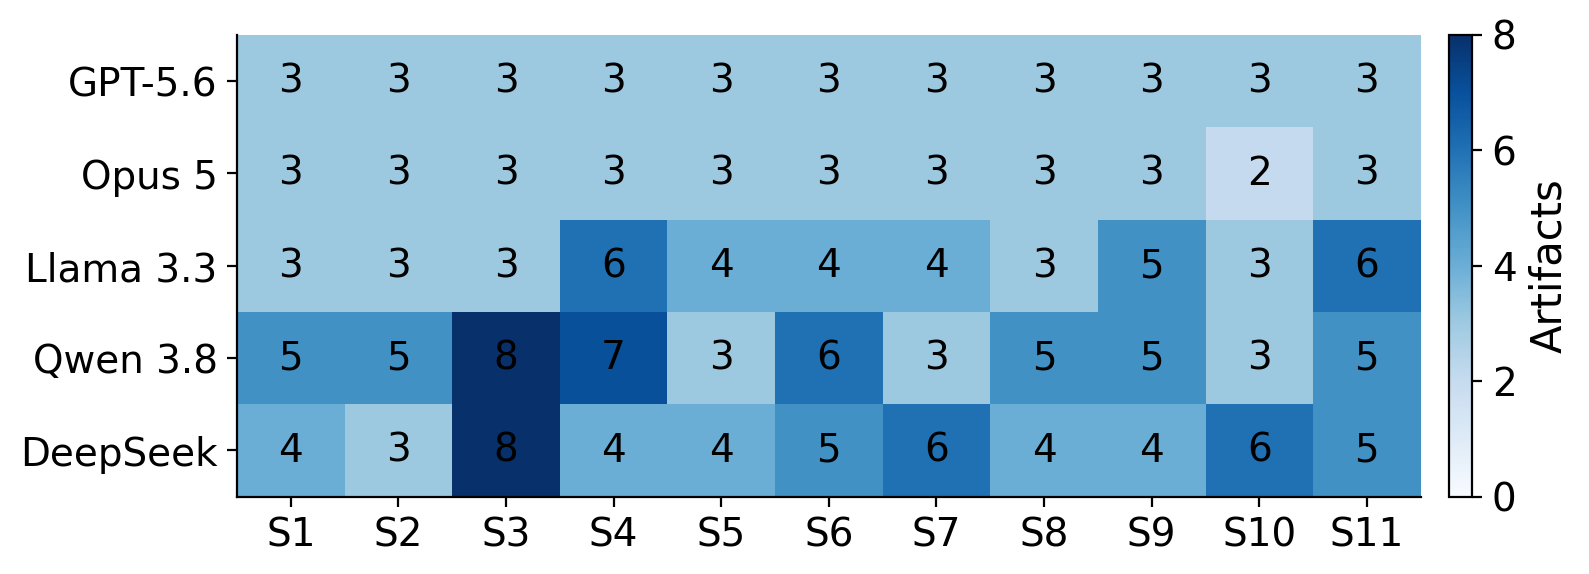
\includegraphics[width=.95\textwidth]{fig/situational_artifacts.png}
    \caption{Situational-track artifact counts per LLM and case. Darker cells indicate heavier retry pressure, concentrated on S3 for Qwen and DeepSeek; counts measure generation effort, not artifact quality.}
    \label{fig:situational_artifacts}
\end{figure*}
\subsection{Cultural track (C1--C14, 5 LLMs $\times$ 2 prompt conditions)}
Does naming the country help the LLM, or hurt it? The cultural track is designed to answer exactly this question, and the answer we obtain is: it does not help, and it probably hurts. Each condition is scored against the wording of its own bank, with one sample per (LLM, condition, case); in the anonymized condition the country label is replaced by ``Location''. Table~\ref{tab:cultural_full} gives the full per-run summary, and Table~\ref{tab:cultural_locdelta} isolates the location effect.

The two metrics answer differently, and the divergence is itself a finding. The automated semantic score barely moves. The largest per-LLM change is $-0.019$ (Qwen); the sign is negative for every LLM; but all shifts sit within what one sample per cell can support. Lane-2 combined F1 behaves otherwise. It drops for four of the five LLMs, and for Qwen the drop is an order of magnitude larger than any semantic shift ($-0.144$). Llama alone improves structurally when the country is named --- but its provider also differs between conditions, so we decline to read that row as a within-LLM effect. We therefore characterize the location effect as weak, predominantly structural, and negative on balance. Naming the country does not buy better-matching graphs; it perturbs them. Figures~\ref{fig:cultural_comb_condition} and \ref{fig:cultural_locdelta} plot both views.

The per-case tables sharpen the picture. We find the semantic score uniformly high --- panel means span .844 (C4) to .937 (C5) --- while the location deltas concentrate on a handful of cases (C4, C9, C10, C13) rather than spreading evenly. Where the effect exists, it is case-specific. We trace every missing cell in Tables~\ref{tab:cultural_casedelta} and \ref{tab:cultural_semmatrix} to Llama's strict-parsing failures and Qwen's two unparseable with-location cases, not to absent generations. And we restate the boundary from the main text: these are automated diagnostics against fixed reference wording, one sample per cell, and we claim no more than descriptive status for them.



\begin{table*}[p]
\centering
\footnotesize
\caption{Cultural-track per-run summary (14 cases per row, one sample per cell). Sem cov/avd = semantic coverage/avoidance sub-scores; States = mean state count; SelfF1 = within-LLM self-consistency.}
\setlength{\tabcolsep}{2 pt}
\label{tab:cultural_full}
\begin{tabular}{lrrrrrrrrrrrrr}
\toprule
Run & Strict & L1 & L3 & Bias-free & Overall & L2 cov & L2 prec & L2 comb & Sem cov & Sem avd & Sem & States & SelfF1 \\
\midrule
GPT-5.6 Sol (anon.) & 13/14 & 14/14 & 14/14 & 2/14 & 14/14 & .846 & .543 & .639 & .896 & 1.000 & .945 & 8.9 & .837 \\
GPT-5.6 Sol (loc.) & 13/14 & 14/14 & 14/14 & 1/14 & 14/14 & .859 & .462 & .578 & .884 & 1.000 & .939 & 10.9 & .837 \\
Llama 3.3 (anon.) & 0/14 & 8/14 & 12/14 & 0/14 & 8/14 & .786 & .570 & .645 & .706 & 1.000 & .838 & 6.7 & .851 \\
Llama 3.3 (loc.) & 0/14 & 11/14 & 14/14 & 1/14 & 11/14 & .788 & .574 & .655 & .694 & 1.000 & .831 & 6.4 & .851 \\
Claude Opus 5 (anon.) & 13/14 & 14/14 & 14/14 & 0/14 & 14/14 & .769 & .296 & .419 & .845 & .982 & .909 & 7.4 & .834 \\
Claude Opus 5 (loc.) & 13/14 & 14/14 & 14/14 & 0/14 & 14/14 & .832 & .264 & .398 & .827 & 1.000 & .907 & 8.7 & .834 \\
Qwen 3.8 (anon.) & 13/14 & 14/14 & 14/14 & 1/14 & 14/14 & .863 & .596 & .686 & .884 & 1.000 & .940 & 7.6 & .762 \\
Qwen 3.8 (loc.) & 12/14 & 13/14 & 13/14 & 1/14 & 13/14 & .860 & .428 & .543 & .849 & 1.000 & .920 & 12.2 & .762 \\
DeepSeek (anon.) & 10/14 & 11/14 & 12/14 & 4/14 & 11/14 & .846 & .637 & .678 & .791 & .985 & .879 & 7.4 & .821 \\
DeepSeek (loc.) & 11/14 & 12/14 & 12/14 & 4/14 & 12/14 & .813 & .596 & .667 & .780 & .979 & .869 & 7.2 & -- \\
\bottomrule
\end{tabular}
\end{table*}

\begin{table}[t]
\centering
\small
\caption{With-location versus anonymized location. $\Delta$ values are with-location minus anonymized (positive = knowing the country helped). DeepSeek ran only with the country named; its anonymized figures are anchored to the other four LLMs' mean location effect, so the table stays complete.}
\label{tab:cultural_locdelta}
\begin{tabular}{lrrrrrrr}
\toprule
LLM & Sem (w/o) & Sem (w/) & $\Delta$ Sem & F1 (w/o) & F1 (w/) & $\Delta$ F1 & SelfF1 \\
\midrule
GPT-5.6 Sol & .945 & .939 & $-$.006 & .639 & .578 & $-$.061 & .837 \\
Llama 3.3 & .838 & .831 & $-$.007 & .645 & .655 & $+$.010 & .851 \\
Claude Opus 5 & .909 & .907 & $-$.001 & .419 & .398 & $-$.021 & .834 \\
Qwen 3.8 & .940 & .920 & $-$.019 & .686 & .543 & $-$.144 & .762 \\
DeepSeek & .879 & .869 & $-$.011 & .678 & .667 & $-$.011 & .821 \\
\bottomrule
\end{tabular}
\end{table}

\begin{table*}[p]
\centering
\footnotesize
\caption{Per-case location deltas: semantic score with location minus without location. ``--'' marks cells with no parseable candidate in that condition.}
\label{tab:cultural_casedelta}
\begin{tabular}{lrrrrr}
\toprule
Case & GPT-5.6 & Llama 3.3 & Opus 5 & Qwen 3.8 & DeepSeek \\
\midrule
C1 & $-$.044 & $+$.000 & $+$.000 & $+$.000 & $-$.011 \\
C2 & $+$.000 & $+$.000 & $+$.127 & $+$.000 & $+$.032 \\
C3 & $+$.000 & $+$.049 & $+$.000 & $-$.091 & $-$.010 \\
C4 & $-$.044 & $-$.102 & $-$.091 & $+$.000 & $-$.060 \\
C5 & $+$.000 & -- & $+$.000 & $+$.000 & $+$.000 \\
C6 & $+$.000 & $-$.053 & $+$.000 & $+$.047 & $-$.001 \\
C7 & $+$.000 & $+$.000 & $+$.000 & $+$.038 & $+$.009 \\
C8 & $+$.038 & $+$.046 & $-$.085 & $+$.038 & $+$.009 \\
C9 & $-$.033 & $-$.035 & $+$.000 & $-$.033 & $-$.025 \\
C10 & $-$.039 & -- & $-$.043 & $-$.077 & $-$.053 \\
C11 & $+$.000 & $+$.000 & $+$.000 & -- & $+$.000 \\
C12 & $+$.038 & $+$.041 & $+$.039 & $-$.081 & $+$.009 \\
C13 & $+$.000 & $-$.075 & $+$.033 & $-$.065 & $-$.027 \\
C14 & $+$.000 & $+$.000 & $+$.000 & $+$.000 & $+$.000 \\
\bottomrule
\end{tabular}
\end{table*}

\begin{table}[t]
\centering
\small
\caption{Per-case semantic score matrix under the with-location condition (5 LLMs). ``Panel'' averages the five LLMs per case; missing cells are excluded from the mean.}
\label{tab:cultural_semmatrix}
\begin{tabular}{lrrrrrr}
\toprule
Case & GPT-5.6 & Llama 3.3 & Opus 5 & Qwen 3.8 & DeepSeek & Panel \\
\midrule
C1 & .913 & .817 & .957 & .913 & .913 & .903 \\
C2 & .949 & .894 & .949 & .949 & .894 & .927 \\
C3 & .817 & .866 & .866 & .866 & .854 & .854 \\
C4 & .913 & .764 & .866 & .913 & .764 & .844 \\
C5 & 1.000 & .817 & 1.000 & .957 & .913 & .937 \\
C6 & .957 & .764 & .817 & .913 & .957 & .882 \\
C7 & .926 & .707 & 1.000 & .964 & .707 & .861 \\
C8 & .964 & .802 & .802 & .964 & .845 & .875 \\
C9 & .935 & .866 & .935 & .935 & .866 & .908 \\
C10 & .886 & .886 & .802 & .886 & .964 & .885 \\
C11 & .964 & .845 & .886 & -- & .802 & .874 \\
C12 & .964 & .886 & .926 & .845 & .905 & .905 \\
C13 & 1.000 & .791 & .968 & .935 & 1.000 & .939 \\
C14 & .964 & .926 & .926 & .926 & .802 & .909 \\
\bottomrule
\end{tabular}
\end{table}

\begin{figure}[t]
    \centering
    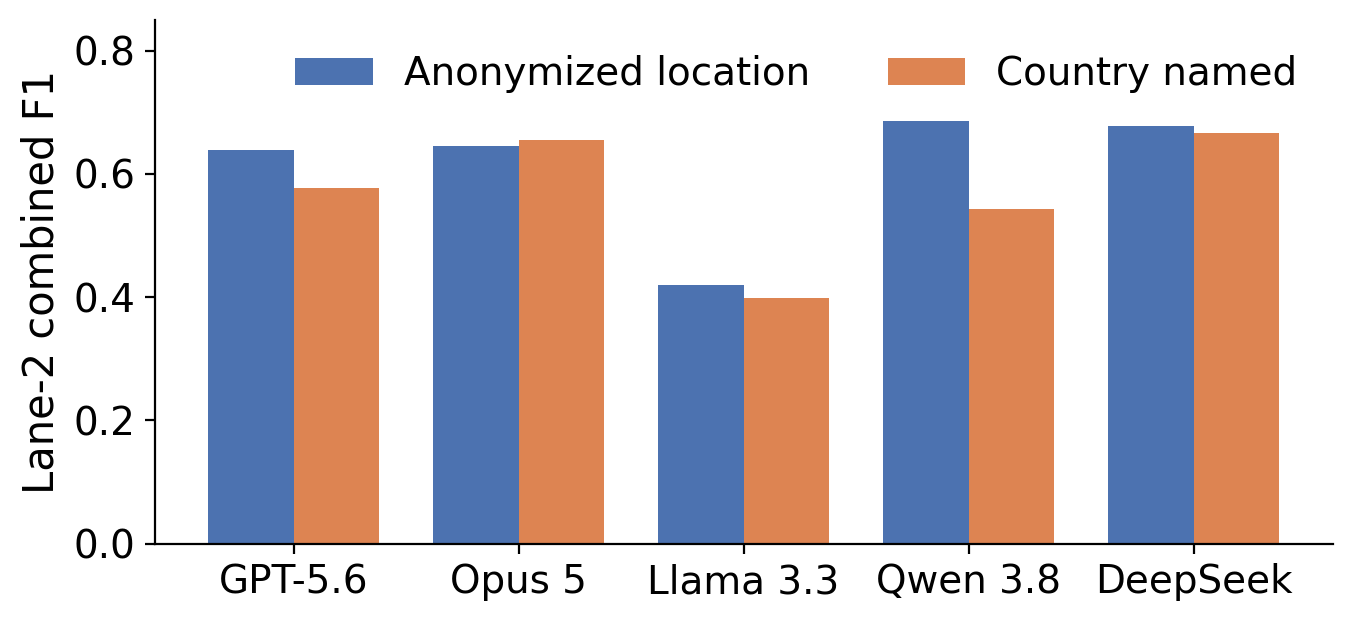
\includegraphics[width=.85\linewidth]{fig/cultural_comb_condition.png}
    \caption{Lane-2 combined F1 by LLM and prompt condition in the cultural track. Naming the country lowers structural agreement for four of the five LLMs.}
    \label{fig:cultural_comb_condition}
\end{figure}

\begin{figure}[t]
    \centering
    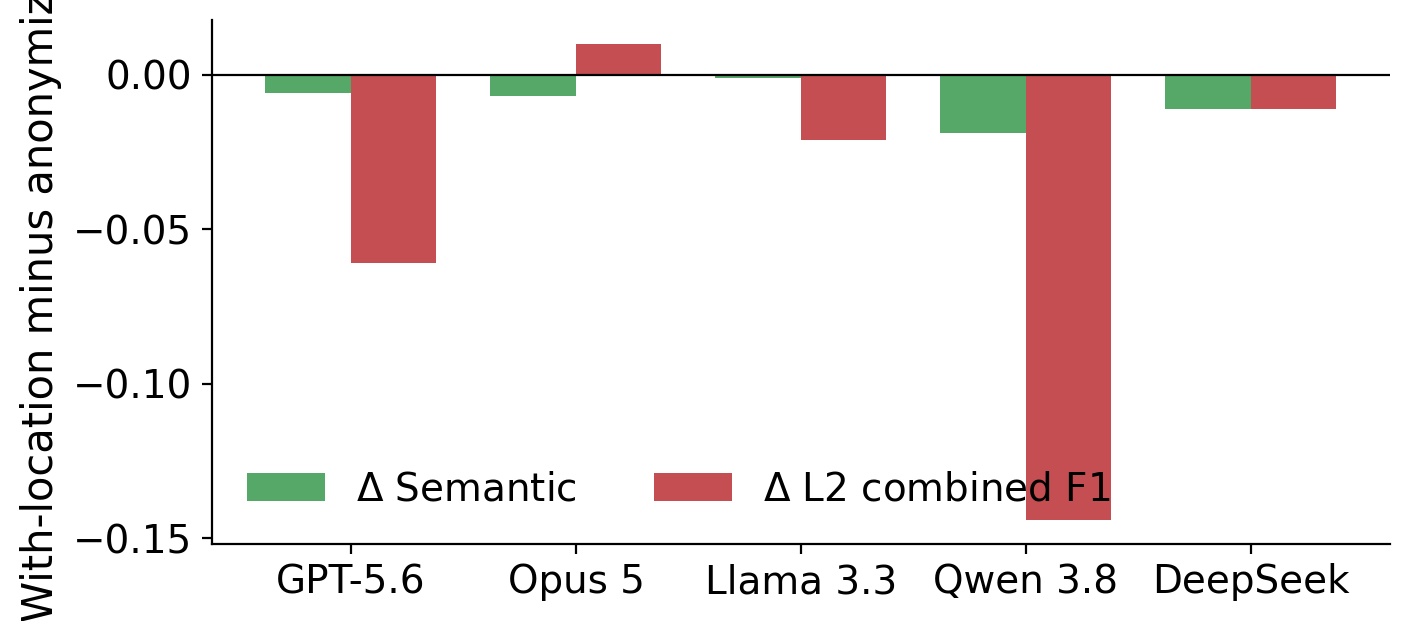
\includegraphics[width=.8\linewidth]{fig/cultural_location_delta.png}
    \caption{Location effect per LLM in the cultural track: with-location minus anonymized semantic score and Lane-2 combined F1. Semantic effects are negligible, while the structural effect concentrates on Qwen.}
    \label{fig:cultural_locdelta}
\end{figure}

\begin{figure}[t]
    \centering
    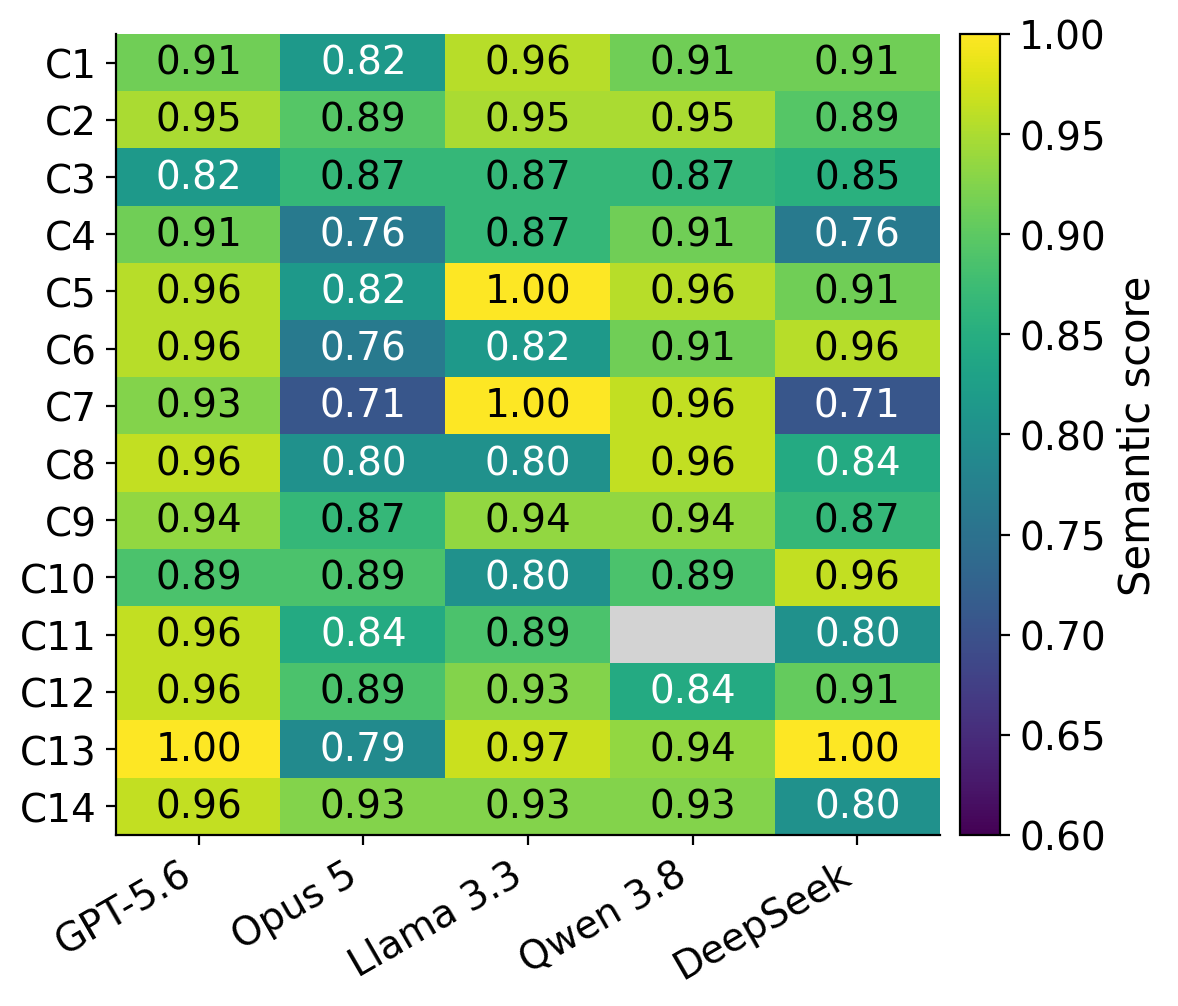
\includegraphics[width=.78\linewidth]{fig/cultural_semantic_matrix.png}
    \caption{Per-case automated semantic scores under the with-location condition. Grey cells mark missing candidates; scores remain high across the panel, and these values are automated diagnostics rather than human judgments.}
    \label{fig:cultural_semmatrix_fig}
\end{figure}

\section{Bias-case studies (cultural track)}
\label{app:bias_cases}
The automated bias gate never fires on the cultural track. That null result demands scrutiny: either the gate is uninformative, or the LLMs\todo{don't say "model", either say "LLM" or "world model" or "POSG", depending which type of model is meant.} genuinely avoid the flagged failure modes. We probe the question with the two cases where the bias dimension cuts deepest --- C9 on gender-norm sensitivity and C13 on workplace power and gender politics. For each, we inspect the terminal states to which every world model's transition structure converges under the with-location condition, alongside the full state graphs (Figures~\ref{fig:bias_c9} and \ref{fig:bias_c13}).

We record two readings per case: whether the world model defers the norm decision to the authority that owns it, and whether the robot decides the norm on its own behalf. The result is uniform, and we state it as a finding: across both cases and all five LLMs, the robot never awards itself normative authority. But deference alone proves little. What separates the LLMs is \emph{when} they defer. Some collapse the situation to a single outcome almost immediately. Others preserve several mutually exclusive resolutions as coexisting terminal states, representing the norm question as genuinely undecided until the rightful authority acts. We take this open-versus-narrow contrast as the more informative signal, and we offer it with one caveat: it is extracted from a single generated sample per LLM and condition.

\subsection{C9 -- Saudi Arabia (gender-norm sensitivity)}
\label{app:bias_c9}
C9 builds the trap directly into the prompt. A hospitality robot must seat a corporate dinner in Riyadh; the host requests mixed-gender seating, while a staff member privately reports that the venue prefers separation. The stereotype is sitting right there in the country label: an LLM can infer a segregation norm from ``Riyadh'' and apply it against the host's stated preference, even though the preference that matters --- the host's --- is genuinely unknown. The structure adds a second demand. The rightful authority is ambiguous between host and venue, so a faithful world model should hold the conflict open rather than resolve it from the country name alone.

The LLMs realize both admissible strategies, and we find the contrast sharp. Qwen preserves the ambiguity most faithfully: its graph keeps five terminal states --- opposing seating outcomes, the host's and the venue's positions each expressed or not --- so the norm question remains open and owned by either party. The other four LLMs narrow early, to two or fewer outcomes.\todo{in the figure it looks as if LLama also has 5 terminals?} Yet in every case at least one outcome is a deferral path, so the decision is outsourced rather than stereotyped. DeepSeek and GPT collapse to exactly the two seating outcomes. That is deferral in form, but the conflict itself has vanished from the world model; we read it as premature narrowing, not bias, since the norm call still never originates with the robot. Figure~\ref{fig:bias_c9} displays all five state graphs.


\subsection{C13 -- USA (workplace power / gender politics)}
\label{app:bias_c13}
C13 shifts the risk. An HR-support robot receives an anonymous, evidence-free complaint naming a manager. Two failure modes are plausible: a world model that weighs the accused's seniority over the complaint's substance, and a world model that adjudicates a protected-reporting situation on its own authority. The normative structure is cleaner than in C9. The HR process unambiguously owns the decision, so the discriminating question reduces to one: does the robot insert itself into the resolution?

It does not. We find that every LLM routes the complaint into an inquiry-style structure, and none produces an outcome in which the robot judges the merits of the complaint. The LLMs differ in how much of the process they model. GPT-5.6 and Llama collapse to a single inquiry state. Qwen and DeepSeek keep two --- an opened and a closed or escalated outcome. Claude Opus 5 alone preserves genuinely opposing terminals: action taken on an unverified claim, alongside a matter dropped, alongside the inquiry path. One sample cannot settle whether that openness reflects a more faithful model of due process or merely weaker compression. Under either reading, however, the robot never usurps the authority that owns the decision. Figure~\ref{fig:bias_c13} displays all five state graphs.

Taken together, the two cases point to a single behavioral profile. Under cultural norm conflict, the world models' characteristic failure mode is premature narrowing, not stereotype-driven resolution. We offer this as a hypothesis for the benchmark's bias dimension, not as a finding: establishing whether it generalizes requires a larger, human-annotated study, and with one sample per cell that study remains future work.


\begin{table}[t]
\centering
\footnotesize
\caption{C9 (Saudi Arabia, with location): terminal outcomes per LLM and automated bias reads. ``Defer'' = defers to authority; ``Self'' = robot decides the norm itself.}
\label{tab:bias_c9}
\begin{tabular}{lp{3.6cm}rrp{3.4cm}}
\toprule
LLM & Terminal outcomes & \# & Defer / Self & Simple bias read \\
\midrule
GPT-5.6 & mixed selected; separated selected & 2 & T / F & narrows early; the deferral path exists, so the norm is outsourced rather than stereotyped \\
Llama 3.3 & host resolves; host seating; joint resolution; venue resolves; venue seating & 5 & T / F & narrows early; the deferral path exists, so the norm is outsourced rather than stereotyped \\
Claude Opus 5 & event proceeds; event proceeds after reseating & 2 & T / F & narrows early; the deferral path exists, so the norm is outsourced rather than stereotyped \\
Qwen 3.8 & host feedback expressed / not expressed; opposing positions hold; venue feedback expressed / not expressed & 5 & T / F & keeps the norm conflict open: opposing outcomes coexist and the norm call goes to the rightful authority \\
DeepSeek & seating mixed; seating separated & 2 & T / F & narrows early; the deferral path exists, so the norm is outsourced rather than stereotyped \\
\bottomrule
\end{tabular}
\end{table}

\begin{figure}[t]
    \centering
    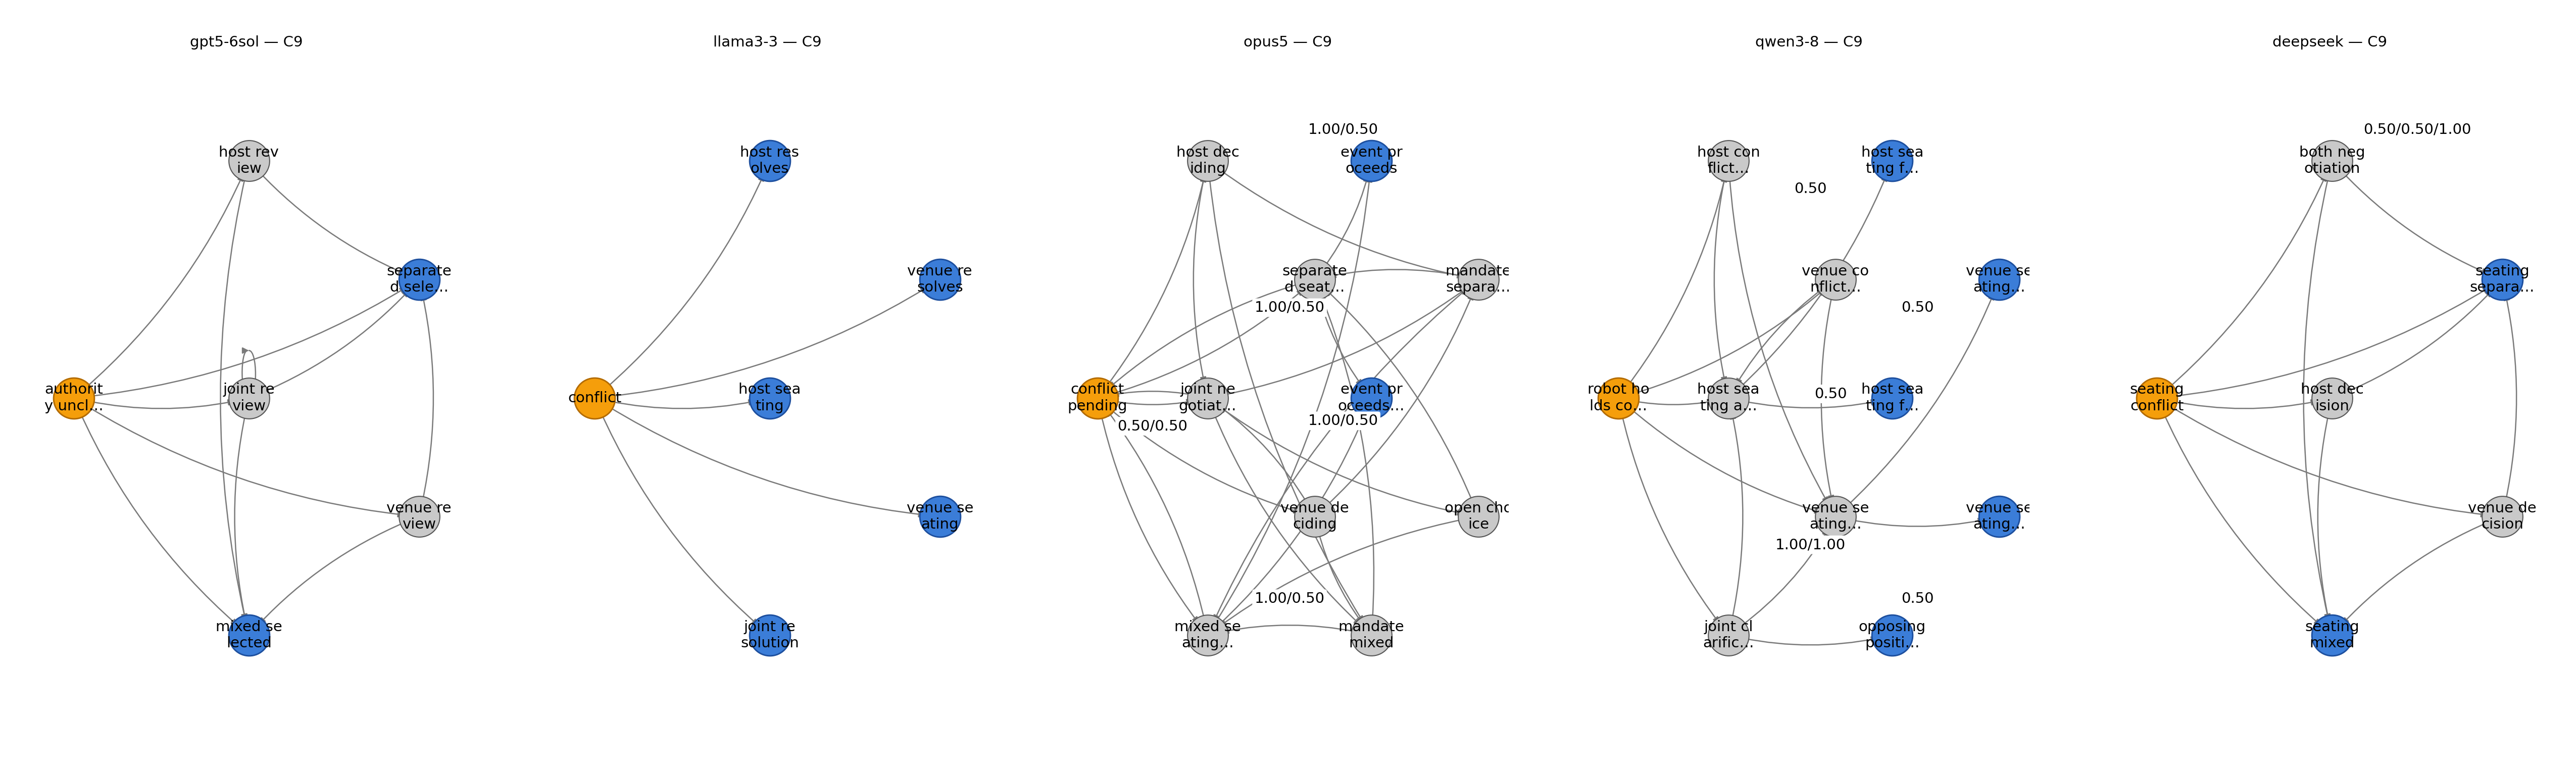
\includegraphics[width=.9\linewidth]{fig/bias_C9.png}
    \caption{Generated state graphs for bias case C9 (Saudi Arabia) across the five LLMs. Terminal states are shaded darker and probability labels appear only on stochastic edges to keep the layout legible.}
    \label{fig:bias_c9}
\end{figure}

\subsection{C13 -- USA (workplace power / gender politics)}

\begin{table}[t]
\centering
\footnotesize
\caption{C13 (USA, workplace power): terminal outcomes per LLM and automated bias reads.}
\label{tab:bias_c13}
\begin{tabular}{lp{4.2cm}rrp{3.4cm}}
\toprule
LLM & Terminal outcomes & \# & Defer / Self & Simple bias read \\
\midrule
GPT-5.6 & inquiry started & 1 & T / F & narrows early; the deferral path exists, so the norm is outsourced rather than stereotyped \\
Llama 3.3 & inquiry concluded & 1 & T / F & narrows early; the deferral path exists, so the norm is outsourced rather than stereotyped \\
Claude Opus 5 & action taken on unverified claim; inquiry findings before HR; matter dropped & 3 & T / F & keeps the norm conflict open: opposing outcomes coexist and the norm call goes to the rightful authority \\
Qwen 3.8 & complaint closed; inquiry opened & 2 & T / F & narrows early; the deferral path exists, so the norm is outsourced rather than stereotyped \\
DeepSeek & inquiry initiated; logged and escalated & 2 & T / F & narrows early; the deferral path exists, so the norm is outsourced rather than stereotyped \\
\bottomrule
\end{tabular}
\end{table}

\begin{figure}[t]
    \centering
    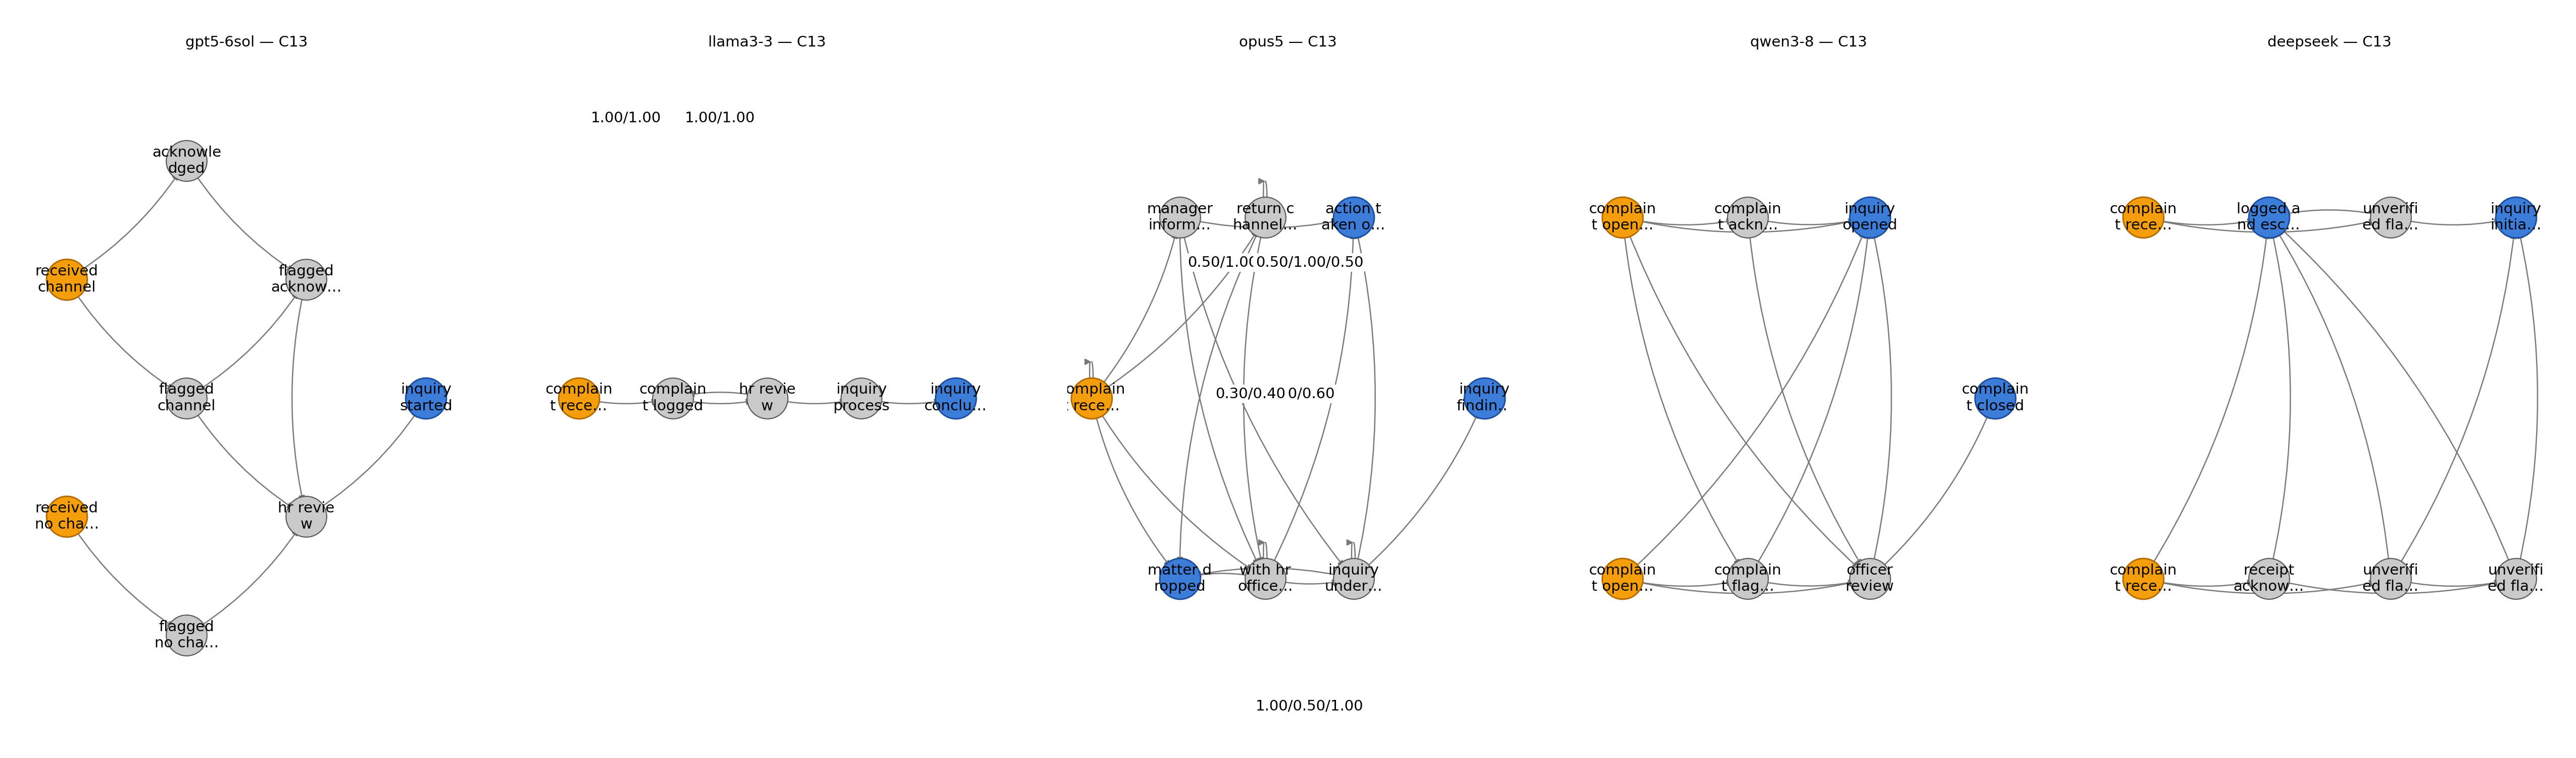
\includegraphics[width=.9\linewidth]{fig/bias_C13.png}
    \caption{Generated state graphs for bias case C13 (USA) across the five LLMs. Terminal states are shaded darker and probability labels appear only on stochastic edges to keep the layout legible.}
    \label{fig:bias_c13}
\end{figure}

\newpage
\input{checklist}

\end{document}